% Document class (KOMA Script)
\documentclass[
	a4paper, 10pt,
	DIV=9, BCOR=5mm,
	parskip,
	numbers=noenddot,
	listof=totoc,
	bibliography=totoc,
]{scrreprt}
\usepackage[utf8]{inputenc}
\usepackage[ngerman]{babel}
\usepackage[babel,german=quotes]{csquotes}
\usepackage[T1]{fontenc}
\usepackage[onehalfspacing]{setspace} % 1.5 line spacing
\AfterTOCHead{\singlespacing}

\pdfobjcompresslevel=0

% "Fix" for KOMA script warning about floats
\usepackage{scrhack}

% Fonts (Palatino and Inconsolata)
% \usepackage{libertine}
\usepackage[sc]{mathpazo}
% \linespread{1.05} % Recommendation for this font
\usepackage[T1]{fontenc}
\usepackage{inconsolata}

% Setting serif-font for headings
% (sans-serif by default)
\addtokomafont{chapter}{\rmfamily}
\addtokomafont{section}{\rmfamily}
\addtokomafont{subsection}{\rmfamily}
\addtokomafont{disposition}{\rmfamily}

% Prevent orphans and widows
\usepackage[all]{nowidow}

% Footnotes in tables
\usepackage{tablefootnote}

% Continuous footnote numbers
\usepackage{chngcntr}
\counterwithout{footnote}{chapter}

% Blockquotes
\usepackage{etoolbox}
\patchcmd{\quote}{\rightmargin}{\leftmargin 4em \rightmargin}{}{}
\newenvironment{itquote}{\bigskip\begin{quote}\itshape}{\end{quote}\bigskip}

% Enumerations
\usepackage{enumitem}

% Figures
\usepackage{graphicx}
\usepackage{subfig}

% Trees
% \usepackage{qtree}
\usepackage{tikz}
\usepackage{tikz-qtree}

% Availability circles
\definecolor{x3domc}{RGB}{0,83,180}
\definecolor{webglc}{RGB}{153,0,0}
\newcommand{\xpie}[1]{%
	\begin{tikzpicture}
		\draw[x3domc] (0,0) circle (0.6ex);\fill[rotate=90,fill=x3domc] (0.6ex,0) arc (0:-#1*90:0.6ex) -- (0,0) -- cycle;
	\end{tikzpicture}%
}
\newcommand{\wpie}[1]{%
	\begin{tikzpicture}
		\draw[webglc] (0,0) circle (0.6ex);\fill[rotate=90,fill=webglc] (0.6ex,0) arc (0:-#1*360:0.6ex) -- (0,0) -- cycle;
	\end{tikzpicture}%
}

% Tables
\usepackage{booktabs}
\usepackage{tabularx}
\newcolumntype{Y}{>{\centering\arraybackslash}X}
\renewcommand{\arraystretch}{1.3}

% Captions
\usepackage[font=small]{caption}
% Overwriting caption labels
\addto\captionsngerman{
	\renewcommand{\figurename}{Abb.}
	\renewcommand{\tablename}{Tab.}
}

% Code listings
\usepackage[outputdir=build]{minted}
\setlength\partopsep{-\topsep}
\newminted{html}{linenos, fontsize=\footnotesize, tabsize=4, baselinestretch=1}
\newminted{js}{linenos, fontsize=\footnotesize, tabsize=4, baselinestretch=1}
\newmintedfile[htmlinput]{html}{linenos, fontsize=\footnotesize, tabsize=4, baselinestretch=1}
\newmintedfile[jsinput]{javascript}{linenos, fontsize=\footnotesize, tabsize=4, baselinestretch=1}
\newmintedfile[jsginput]{javascript}{linenos, fontsize=\footnotesize, tabsize=4, baselinestretch=1,gobble=4}
\newmintedfile[jsgginput]{javascript}{linenos, fontsize=\footnotesize, tabsize=4, baselinestretch=1,gobble=8}
\renewcommand{\theFancyVerbLine}{\scriptsize{\arabic{FancyVerbLine}}}
\renewcommand\listoflistingscaption{Quelltext-Listings}

% TOC
\usepackage{tocstyle}
\usetocstyle{allwithdot}
% Solve overfull hbox problem
\makeatletter
\renewcommand{\@pnumwidth}{2em}
\renewcommand{\@tocrmarg}{3em}
\makeatother

% Write the word "Appendix" in front of every appendix entry
\providecommand*{\appendixmore}{}
\newcommand*{\SavedOriginaladdchaptertocentry}{}
\appto\appendixmore{%
	\let\SavedOriginaladdchaptertocentry\addchaptertocentry
	\renewcommand*{\addchaptertocentry}[2]{%
		\ifstr{#1}{}{%
			\SavedOriginaladdchaptertocentry{}{#2}%
		}{
			\SavedOriginaladdchaptertocentry{}{\appendixname~#1:\enskip#2}%
		}%
	}%
}

% Links in TOC
\usepackage[plainpages=false,hidelinks]{hyperref}
\hypersetup{
    colorlinks,
    citecolor=black,
    filecolor=black,
    linkcolor=black,
    urlcolor=black
}

% BibLaTex (Literature)
\usepackage[backend=biber,sortlocale=de_DE,defernumbers=true]{biblatex}
\addbibresource{literatur.bib}
\renewcommand{\bibfont}{\normalfont\small}
\DefineBibliographyStrings{ngerman}{
	andothers = {et\addabbrvspace al\adddot},
}

\title{Darstellung interaktiver 3D-Grafik im Webbrowser}
\author{Jonathan Gruber}
\date{\today}

\begin{document}
	% Numbering is invisible, but required for hyperref package
	\pagenumbering{Roman}

	\newcommand{\titel}{Darstellung interaktiver\\[0.5ex]3D-Grafik im Webbrowser}
\newcommand{\art}{Bachelorarbeit}
\newcommand{\ziel}{Bachelor of Science}
\newcommand{\fakultaet}{Elektrotechnik und Informatik}
\newcommand{\autor}{Jonathan Gruber}
\newcommand{\studiengang}{Informatik}
\newcommand{\matrikelnr}{31222}
\newcommand{\erstgutachter}{Prof. Dr. rer. nat. Franz Regensburger}
\newcommand{\zweitgutachter}{Prof. Dr. rer. nat. Thomas Grauschopf}
\newcommand{\schule}{Technische Hochschule Ingolstadt}
\newcommand{\instit}{ercas GmbH & Co. KG}
\newcommand{\institbetreuer}{Ulf Schoedel}
\newcommand{\jahr}{2014}
\newcommand{\ort}{Ingolstadt}
\newcommand{\logo}{res/thi_logo.pdf}

	\begin{titlepage}

	\phantom{tmpText}

	\vspace{1cm}

	\begin{figure}[h!]
		\centering
		\includegraphics[height=2.3cm]{\logo}
	\end{figure}

	\begin{center}

		\vspace{1cm}

		\textbf{{\large \art} \\[3ex]
		{\LARGE \titel} \\[8ex]
		Zur Erlangung des akademisches Grades eines \\
		\ziel \\[2ex]
		%
		\vfill
		%
		angefertigt von \\
		\autor} \\[2ex]
		%
		\vfill
		%
		Fakultät: \fakultaet \\
		Studiengang: \studiengang \\[2ex]
		%
		\vfill
		%
		% \textbf{Betreuer}: Ulf Schoedel\\[4ex]
		\begin{tabular}{ll}
			Erstprüfer & \erstgutachter\\
			Zweitprüfer & \zweitgutachter
		\end{tabular} \\[2ex]
		%
		\vfill
		%
		ausgegeben am 01. Juli 2014 \\
		abgegeben am 04. August 2014
		% Max. 3 Tage Abweichung!
	\end{center}
\end{titlepage}


	% TOC
	\setcounter{tocdepth}{2}
	\tableofcontents

	% Remove page numbering in multipage toc
	\thispagestyle{empty}
	\addtocontents{toc}{\protect\thispagestyle{empty}}

	\clearpage
	\pagenumbering{arabic}

	\chapter{Das World Wide Web als Anwendungsplattform der Zukunft}
\label{CHAP:INTRODUCTION}

Durch die zunehmend größere Verbreitung moderner Webstandards wie HTML5 und damit assoziierter Technologien hat sich das World Wide Web (WWW) von einem ehemals simplen Dokumentenbetrachtungssystem zu einer Plattform für vielfältige \emph{Rich Internet Applications} (RIA) entwickelt \autocite{Taivalsaari:2001:Saga_continues}. \textcite{Anttonen:2011:TWR:1982185.1982357} unterteilen diese Entwicklung in drei grobe Phasen:

Während das Web zu Anfang aus statischen, textorientierten HTML-Dokumente bestand, leitet das Aufkommen JavaScripts 1995 die zweite Phase mit immer mehr interaktiven Elementen ein. Proprietäre, weit verbreitete Browser-Plugins wie \emph{Flash}, \emph{Shockwave} und \emph{Quicktime} ermöglichen zusätzlich zu unbewegten Bildern nun auch Animationen und die Einbettung von Video- und Audio-Inhalten.\newline
Die dritte Stufe stellt schließlich den derzeitigen Übergang zu hochinteraktiven Web-""Anwendungen dar, die klassischen Desktop-""Applikationen in ihrem Nutzererlebnis (\emph{User Experience}) immer mehr ähneln.
\textcite{Taivalsaari:2011:Death_of_Binary_Software} vertreten in ihrer Publikation \enquote{\emph{The Death of Binary Software: End User Software Moves to the Web}} die These, dass konventionelle Software zukünftig in immer größerem Maße durch webbasierte Applikationen ersetzt werde. Googles Linux-basiertes Betriebssystem \emph{Chrome OS} ist dafür ein gutes Beispiel. Nahezu alle Anwendungsprogramme werden hier im Webbrowser Chrome ausgeführt.
Zahlreiche in den letzten Jahren aufgekommene Standards wie \emph{Web Storage}, \emph{Web Sockets} und \emph{Media Capture} unterstreichen diesen Bedeutungszuwachs von Web-Anwendungen und stützen die Prognose Taivalsaaris. Ein Bereich, der sich bisher noch kaum im Web etablieren konnte und nach wie vor in erster Linie konventioneller Client-Software vorbehalten ist, ist die hardwarebeschleunigte Darstellung von 3D-Grafik.

In seinem Artikel \enquote{\emph{Is 3D Finally Ready for the Web?}} aus dem Jahr 2010 behandelt Sixto Ortiz Jr. die Fragestellung, ob das Web nach zahlreichen gescheiterten Anläufen inzwischen gerüstet sei, auch diese \enquote{letzte Bastion} \autocite{Taivalsaari:2011:Death_of_Binary_Software} traditioneller Software abzubilden. Der Autor analysiert hierfür den damaligen Stand webbasierter 3D-Grafik und kommt zum Schluß, dass es immer noch viele Hürden gibt, die einen Durchbruch dieser Technik verhindert. Er sah hierbei die Notwendigkeit von Browser-Plugins und den Mangel an Standardisierung als hauptsächliche Probleme.
	\chapter{Motivation und Aufbau der Arbeit}
\label{CHAP:MOTIVATION}

Mit der Veröffentlichung des Internet Explorers 11 im Herbst 2013 \autocite{MS_RELEASE_IE11} ist der freie Grafikstandard \emph{Web Graphics Library} (WebGL) erst kürzlich in den Webbrowser von Microsoft eingezogen. Hierdurch sind die Grundvoraussetzungen für die Plugin-freie Darstellung hardwarebeschleunigter 3D-""Grafik nun in nahezu allen aktuellen Desktop-Browsern gegeben.
Auch im mobilen Bereich ist derzeit eine neue Dynamik zu erkennen. So kündigte Apple im Juni 2014 die Integration von WebGL in ihre mobile Plattform \emph{iOS 8} an \autocite{APPLE_WWDC_2014_WEBGL}. Der Einflussbereich dieser Technologie nimmt damit weiter zu und die Etablierung von 3D-""Grafik im \emph{World Wide Web} scheint in greifbare Nähe gerückt.

Vier Jahre nach Ortiz Artikel soll dessen Grundfrage, ob das WWW bereit sei für die dritte Dimension, erneut aufgegriffen werden. Gegenstand dieser Arbeit ist davon ausgehend die Evaluation der zwei offenen Grafikstandards  WebGL und X3D bezüglich ihrer Eignung für die Realisierung interaktiver 3D-""Grafik im Webbrowser. Hierfür werden die zwei Technologien hinsichtlich verschiedener Kriterien gegenüber gestellt.

Die Arbeit ist wie folgt strukturiert: Zunächst werden einige elementare Grundbegriffe und Prinzipien der Computergrafik erläutert, um das Verständnis der nachfolgenden Ausführungen zu erleichtern. Daraufhin wird die behandelte Anwendungsdomäne der betrachteten Klasse von 3D-""Anwendungen konkretisiert und der thematische Umfang der Untersuchung eingegrenzt. Ausgehend von exemplarischen Anwendungsfällen werden anschließend Ziele der Evaluation und Anforderungen einer solchen 3D-""Anwendung spezifiziert. Um den grundsätzlichen Aufbau und die Funktionsweise der zwei betrachteten Technologien aufzuzeigen, werden diese im Anschluss daran im Detail beleuchtet. Dasselbe Beispiel verdeutlicht jeweils die paradigmatischen Besonderheiten beider Ansätze. Schließlich wird die Evaluation ausgehend von den zuvor spezifizierten Kritieren durchgeführt. Hierfür werden zum einen die Ergebnisse automatisierter Tests betrachtet und zum anderen solche Aspekte untersucht, die nur schwer quantifiziert werden können. Zuletzt werden die Ergebnisse hinsichtlich der Zielvorgabe bewertet und ein Fazit gezogen.

	\chapter{Begrifflichkeit und computergrafische Grundlagen}
\label{CHAP:FUNDAMENTALS}

Bevor die Bewertungskriterien der späteren Evaluation spezifiert werden, sollen zunächst einige häufig vorkommende Fachbegriffe und elementare Konzepte der Computergrafik erläutert werden, um das Verständnis der weiteren Ausführungen zu erleichtern.

\section{Grundbegriffe}
\label{SEC:BASIC_CONCEPTS}

Ein durch das \emph{World Wide Web Consortium} (W3C) definierter Standard für den Zugriff und die Manipulation von HTML- und XML-Dokumenten ist das \textbf{Document Object Model} (DOM). Die durch diese Spezifikation definierte Programmierschnittstelle ermöglicht das Traversieren, Hinzufügen, Ändern und Entfernen von DOM-Elementen, sodass ein Dokument vollständig dynamisch bearbeitet werden kann \autocite{W3C_DOM_CORE_3}. Das World Wide Web Consortium ist ein internationales Gremium zur Standardisierung von Techniken rund um das WWW \autocite{W3C_ABOUT}.

Ein Sammelbegriff für sämtliche Technologien rund um die Darstellung von 3D-""Computergrafik im World Wide Web ist \textbf{Web3D}. Dieses beinhaltet sowohl traditionelle Ansätze auf Basis von Browser-Plugins als auch jüngst aufgekommene native Umsetzungen.
Die Bildsynthese -- oder gängiger: das \textbf{Rendering} -- bezeichnet die Erzeugung eines zweidimensionalen Einzelbilds, welches ausgehend von einer virtuellen 3D-""Darstellung berechnet wird. Dieses Bild kann im Anschluss auf dem Bildschirm oder einem anderen Ausgabemedium angezeigt werden.

\begin{figure}[htb]
	\centering
	\subfloat[Polygonnetz]{
		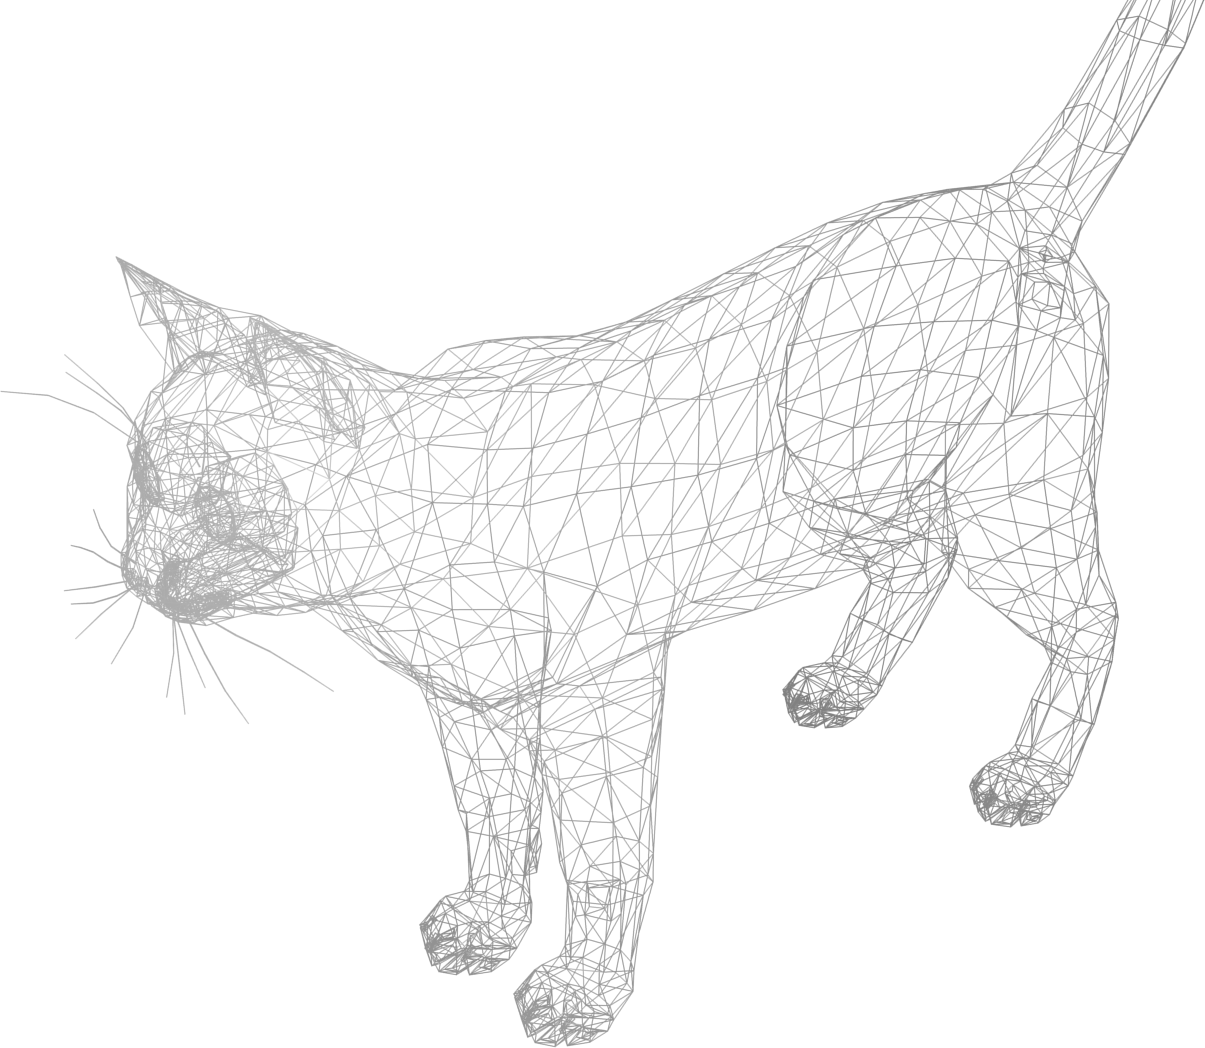
\includegraphics[width=0.31\textwidth]{kap2/figures/cat-wireframe.png}
		\label{FIG:3DMODEL_WIREFRAME}
	}
	\hfill
	\subfloat[Flat-Shading]{
		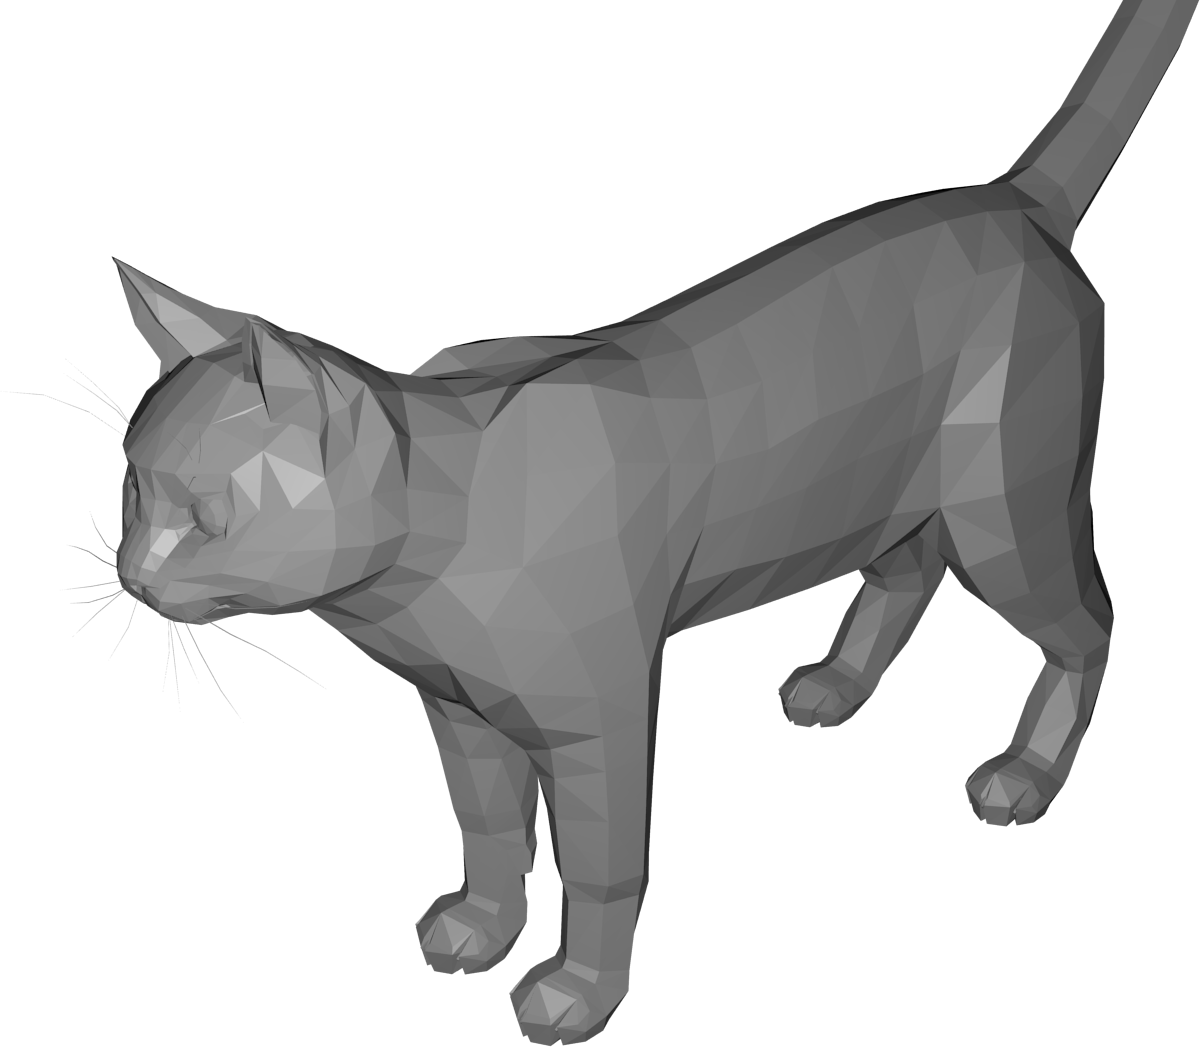
\includegraphics[width=0.31\textwidth]{kap2/figures/cat-flat-shading.png}
		\label{FIG:3DMODEL_FLAT_SHADING}
	}
	\hfill
	\subfloat[Smooth-Shading]{
		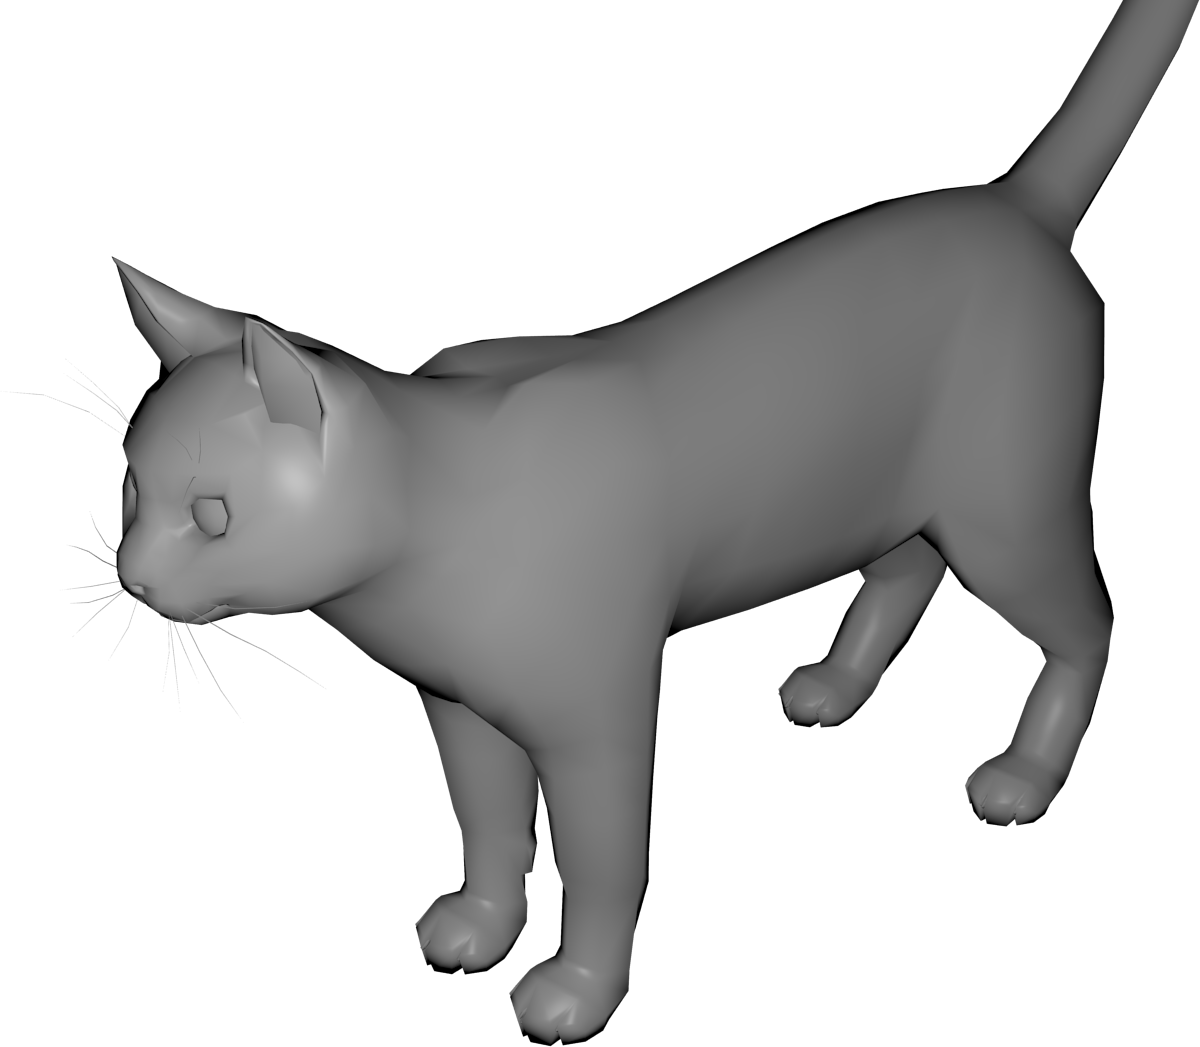
\includegraphics[width=0.31\textwidth]{kap2/figures/cat-smooth-shading-lambert-phong.png}
		\label{FIG:3DMODEL_SMOOTH_SHADING}
	}
	\caption{Verschiedene Darstellungen eines 3D-Modells.}
	\label{FIG:3DMODELS_SHADING}
\end{figure}

Abbildung \ref{FIG:3DMODELS_SHADING} zeigt verschiedene Darstellungen eines \textbf{3D-""Modells}. Ein solches Modell ist die mathematische Repräsentation eines dreidimensionales Objekts im Raum, definiert durch eine Menge von Punkten (\textbf{Vertices}\footnote{Singular: Vertex.}) Kanten. Wie die linke Figur zeigt, verbinden Kanten die Vertices zu einem Polygonnetz, welches die Seiten (\emph{Faces}) des Objekts formt. Als Polygone dienen in der Computergrafik typischerweise Dreiecke. Diese sind aufgrund der Eigenschaft dass sie stets planar vorliegen, besonders gut für grafische Berechnungen geeignet \autocite{MOZILLA_CONCEPTS_OF_WEBGL}. Weiterhin wird die Orientierung der Polygone durch deren Normalenvektor festgelegt. Diese ist zum einen für Sichtbarkeitsentscheide (\emph{Culling}) wichtig und dient zum anderen der Berechnung von Beleuchtungsmodellen. Unter \textbf{Culling} wird eine Reihe von Algorithmen verstanden, die darüber entscheiden, welche Objekte einer 3D-Szene zu zeichnen sind und welche nicht. Elemente, die komplett außerhalb des sichtbaren Bereichs liegen, müssen beispielsweise nicht betrachtet werden und verursachen so keinen unnötigen Rechenaufwand.

Ein \textbf{Beleuchtungsmodell} stellt das Verfahren dar, welches den Einfluss von Licht in einer 3D-Szene simuliert \autocite[190\psq]{Zeppenfeld:2004}. Hierbei wird zwischen dem lokalen und globalen Beleuchtungsmodell unterschieden. Während Ersteres lediglich den Einfluss der Lichtquellen in einem Punkt der Objektoberfläche berücksichtigt, werden beim globalen Modell auch Reflexion, Transparenzeffekte und Lichtbrechung mit einbezogen.

\begin{figure}[ht]
	\centering
	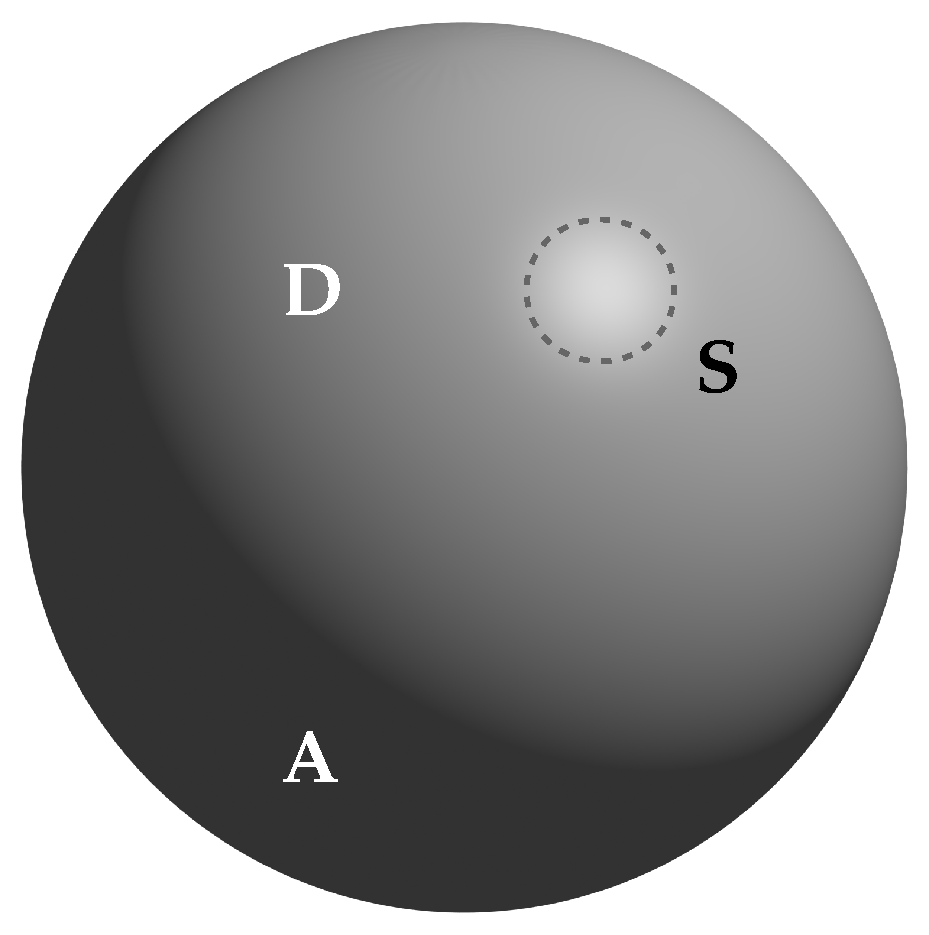
\includegraphics[width=0.25\textwidth]{kap2/figures/illumination-crop.pdf}
	\caption{Ambiente, diffuse und spekulare Beleuchtung.}
	\label{FIG:ILLUMINATION}
\end{figure}

Abbildung \ref{FIG:ILLUMINATION} zeigt wichtige Licht- und Reflexionsmodelle der Computergrafik \autocite[722\psq]{Foley:CG_PRINCIPLES_AND_PRACTICE}. Ambientes Licht (A) kommt aus allen Richtungen und hat somit auf alle Objekte denselben Einfluss, unabhängig von deren Position im Raum. Es sorgt für die Grundhelligkeit einer Szene, sodass selbst im Schatten liegende Objekte nicht tiefschwarz sind, sondern eine Grauschattierung aufweisen. Die diffuse Reflexion (D) führt zu einer gleichmäßigen Reflexion des Lichts in alle Richtungen. Da der Einfallswinkel des Lichts hierbei berücksichtig wird, entsteht ein plastischer Eindruck. Die spekulare oder spiegelnde Reflexion (S) sorgt schließlich für Glanzeffekte (\emph{Highlights}) auf der Materialoberfläche.

Die Abbildungen \ref{FIG:3DMODEL_FLAT_SHADING} und \ref{FIG:3DMODEL_SMOOTH_SHADING} auf der vorherigen Seite zeigen verschiedene Schattierungsverfahren (\textbf{Shading}). Der weit gefasste Begriff \emph{Shading} bezeichnet die Berechnung der Beleuchtung und Materialeigenschaften von Objektoberflächen. Durch Anwendung von \emph{Flat-Shading} (Mitte) wird die Farbe jedes Polygons durch dessen Normale entsprechend des lokalen Beleuchtungsmodells berechnet. Hieraus resultiert eine einheitliche Färbung des gesamten Polygons. Das \emph{Smooth-Shading} (rechts) -- genauer ein sogenanntes \emph{Phong-Shading}\footnote{Benannt nach Erfinder des Verfahrens, dem vietnamesischen Computergrafiker Bui Tuong Phong.} -- führt zu einer glatten Oberfläche, indem die Normalen der Polygone interpoliert werden und die Farbe jedes Pixels hiervon ausgehend erneut durch Anwendung des lokalen Beleuchtungsmodells berechnet wird \autocite[203\psq]{Zeppenfeld:2004}. Das Phong-Verfahren erzeugt weiterhin Glanzeffekte durch spekulare Reflexion (siehe Kopf der Katze in Abbildung \ref{FIG:3DMODEL_SMOOTH_SHADING}).

\begin{figure}[ht]
	\centering
	\small
	\Tree [.{\textbf{Universum}} Lichtquelle [.{Affine Transformation} [.{Modell 1} Geometrie Material ] {Modell 2} ] ]
	\caption{Exemplarischer Szenengraph (unvollständig).}
	\label{FIG:SCENEGRAPH_EXAMPLE}
\end{figure}

Eine in der Computergrafik häufig vorkommende Datenstruktur zur Repräsentation hierarchischer 3D-""Szenen ist der sogenannte \textbf{Szenengraph}. Hierbei handelt es sich um einen gerichteten azyklischen Graph, dessen Wurzelknoten das \emph{Universum}, also die vollständige Szene darstellt. Kindknoten der Wurzel sind Objekte der Szene und können wiederum weitere Elemente enthalten (vgl. Abbildung \ref{FIG:SCENEGRAPH_EXAMPLE}). Transformationen auf einen Knoten werden auf alle Kinder weitervererbt.

\section{Standard-Grafikpipeline}
\label{SEC:STANDARD_GRAPHICS_PIPELINE}

Ein weiteres elementares Konzept nahezu aller heutigen Grafiksysteme ist die sogenannte Grafik- oder Rendering-Pipeline \cite[866-871]{Foley:CG_PRINCIPLES_AND_PRACTICE}. Diese beschreibt die Gesamtheit der Einzelschritte, die nötig sind, um eine virtuelle 3D-""Szene mittels mehrerer Transformationen und Berechnungen auf den zweidimensionalen Bildschirm abzubilden. Die späteren Beispiele der betrachteten Technologien werden diese Konzepte praktisch widerspiegeln.

Der Begriff \enquote{Pipeline} kann analog zu klassischen UNIX-Pipelines gesehen werden und verdeutlicht das Prinzip des Verfahrens: Die Ausgabe einer Operation dient als Eingabe des nächsten Prozesses.
Die Effizienz der grafischen Berechnungen wird hierbei wie in Abbildung \ref{FIG:RENDERING_PIPELINE} angedeutet durch Parallelisierung innerhalb des Grafikprozessors (\emph{Graphics Processing Unit}), dessen Hardware hinsichtlich dieser Anforderung optimiert ist, enorm gesteigert. Vor jedem Schritt muss die Pipeline auf Fertigstellung der vorherigen Berechnung warten. Abbildung \ref{FIG:RENDERING_PIPELINE} zeigt den schematischen Aufbau der Pipeline:

\begin{figure}[hb]
	\centering
	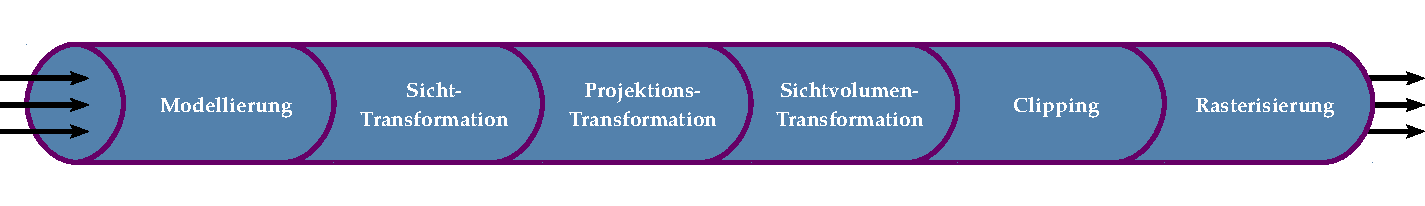
\includegraphics[width=1.0\textwidth]{kap2/figures/rendering-pipeline-crop.pdf}
	\caption{Schematische Darstellung der Standard-Grafikpipeline.}
	\label{FIG:RENDERING_PIPELINE}
\end{figure}

Während die Funktionalität der Pipeline zu Anfang der Hardware-""Entwicklung statisch umgesetzt war (\emph{Fixed-Function-Pipeline}) und nur durch wenige Parameter angepasst werden konnte, sind heutige Implementierungen durch sogenannte \emph{Shader} vollständig programmierbar und weisen eine hohe Flexiblität auf\footnote{Shader-Programme werden in Abschnitt \ref{SEC:WEBGL_SHADER} näher behandelt.}. Die Grafikpipeline kann sowohl in Hardware als auch in Software umgesetzt werden. Hardware-""Implementierungen sind Software-basierten Realisierungen jedoch hinsichtlich der Effizienz und Geschwindigkeit deutlich überlegen und daher zu bevorzugen.

Im Folgenden werden die Einzelschritte der Pipeline erläutert. Die Details der konkreten mathematischen Berechnungen werden hierbei nicht weiter ausgeführt, da sie den Rahmen der vorliegenden Arbeit übersteigen.

\subsection{Modellierung}
Zu Beginn des Verfahrens steht das Laden beziehungsweise die Konstruktion der 3D-Modelle.
Nach der Definition von Eckpunkten (\emph{Vertices}) durch Angabe derer kartesischer Koordinaten werden die Modelle durch Polygone zusammengesetzt. Als Polygone dienen typischerweise Dreiecke aufgrund der bereits genannten Vorteile. Diese werden durch je drei Vertices definiert. Natürlich ist eine manuelle Definition der Geometrie in realen Anwendungsfällen bei komplexen Modellen mit zehntausenden von Vertices ausgeschlossen. Gemeinhin enstammen die geometrischen Daten spezieller 3D-""Model"-lierungs"-software wie \emph{Blender} \autocite{SOFTWARE_BLENDER}, die die Erstellung aufwendiger Modelle erheblich erleichtern.

Die Koordinaten der Vertices liegen zunächst relativ zur \enquote{Modelmitte} in einem lokalen Koordinatensystem vor. Mittels affiner Transformationen können die Modelle im Raum verschoben, skaliert, rotiert und verzerrt werden. Dies wird durch Multiplikation der entsprechenden, homogenen Transformationsmatrix mit allen Punkten des Modells realisiert. Weiterhin können mehrere Transformationen durch Multiplikationen aller beteiligten Matrizen durch eine einzige gleichwertige Modellmatrix $\underline{M}$ ersetzt werden. Da die Matrizenmultiplikation nicht kommutativ ist, ist die Reihenfolge der Operation entscheidend.

Eine Überführung der Modelkoordinaten in sogenannte Weltkoordinaten wird somit durch folgende Berechnung vollzogen. Dabei sei $\vec{v}_i$ der Spaltenvektor der Koordinaten des aktuell betrachteten Vertex.

\begin{figure}[!h]
	\begin{displaymath}
		\sum_{i=0}^{n} \underline{M} * \vec{v}_i
	\end{displaymath}
	\caption{Berechnung der Modelmatrix.}
\end{figure}

\subsection{Sicht-Transformation}

Anschließend wird die Ansicht der Szene mittels mehrerer Parameter festgelegt. Der Aug- oder Beobachtungspunkt, welcher der \enquote{Kamera} der Szene entspricht, wird zunächst im Weltkoordinatensystem platziert. Des Weiteren wird das Zentrum der Betrachtung der (\emph{Look-At}-Punkt) und der Oben-Vektor spezifiziert. Dieser legt die Orientierung der Ansicht fest, indem er die Richtung \enquote{oben} definiert.

All diese Parameter werden innerhalb der Sichtmatrix $\underline{V}$ abgebildet. Durch Multiplikation der Modellmatrix und der Vertices mit der Sichtmatrix erfolgt die Transformation in das sogenannte Sichtkoordinatensystem. Die Welt wird hierdurch relativ zur Kamera verschoben, welche nun im Ursprung liegt.

\begin{figure}[!h]
	\begin{displaymath}
		\sum_{i=0}^{n} \underline{V} * \underline{M} * \vec{v}_i
	\end{displaymath}
	\caption{Berechnung der MV-Matrix.}
\end{figure}

\subsection{Projektions- und Sichtvolumen-Transformation}
Der nächste Schritt ist die Projektion der Darstellung auf einen Einheitswürfel zur Vorbereitung der Bildschirm-Transformation. Hierfür muss zunächst ein Sichtvolumen definiert werden. Dieses grenzt den darzustellenden Bereichs des 3D-""Raums durch Ebenen ein und wird für das spätere \emph{Clipping} benötigt. Um die Darstellungseffizienz zu steigern, werden dabei Objekte außerhalb dieser Abgrenzung verworfen.

Es stehen verschiedene Projektions-Modelle zur Verfügung. Von besonderer Bedeutung sind die orthogonale Parallelenprojektion und die perspektive Projektion.
Bei der Parallelenprojektion wird das Sichtvolumen durch einen Quader beschrieben, welcher mittels Angabe der Dimensionen für die Ausdehnung des Quaders in alle drei Achsen aufgespannt wird. Die spätere Transformation auf den Einheitswürfel ist in diesem Fall mittels einer Skalierung einfach umzusetzen.
Zur Erzielung eines perspektivischen Effekts, also der Größendarstellung von Objekte in Abhängigkeit von deren Entfernung zum Beobachtungspunkt, wird bei der perspektivischen Projektion ein Pyradmidenstumpf (\emph{Frustum}) verwendet. Durch die verzerrende Abbildung des Frustums auf den Einheitswürfel entsteht so die angestrebte kleinere Darstellung weiter entfernter Elemente.

\begin{figure}[!h]
	\begin{displaymath}
		\sum_{i=0}^{n} \underline{P} * \underline{V} * \underline{M} * \vec{v}_i
	\end{displaymath}
	\caption{Berechnung der MVP-Matrix.}
	\label{CALC:MVP_MATRIX}
\end{figure}

Analog zu den vorherigen Schritten wird auch diese Berechnung durch eine Matrixmultiplikation realisiert. Durch Multiplikation der bisherigen Transformationen mit der Projektionsmatrix, welche die Parameter des gewählten Projektionsmodells enthält, wird hierbei die finale Transformation der Vertices erzielt.

Wie Formel \ref{CALC:MVP_MATRIX} zeigt, kann die gesamte Modell-, Sicht- und Projektionstransformation durch das Matrizenprodukt von $\underline{P}$, $\underline{V}$ und $\underline{M}$ realisiert werden. Dieses Gesamtprodukt der Transformation wird als \emph{MVP-Matrix} bezeichnet. Anstatt für jeden Vertex drei teure Matrizenmultiplikationen durchzuführen, kann die Berechnungseffizienz deutlich gesteigert werden, indem jeder der Punkte lediglich mit der MVP-Matrix multipliziert wird.

\subsection{Clipping}

Nachdem bereits Polygone, welche entweder abgewandt (\emph{Backface-Culling}) oder komplett außerhalb des Sichtvolumens liegen (\emph{Frustum-Culling}\footnote{Bei einer perspektivischen Projektion.}), verworfen wurden, ist der nächste Schritt das sogenannte \emph{Clipping}. Dieses Verfahren betrachtet Polygone, welche das Sichtvolumen schneiden und daher nur teilweise gezeichnet werden müssen. Zu diesem Zweck werden die Schnittpunkte des Polygons mit der Abgrenzung berechnet und anhand dessen ein entsprechendes neues Teilpolygon erstellt. Der Algorithmus von \emph{Cohen-Sutherland} ist ein bekanntes Beispiel für die Realisierung dieses Vorgangs.

Häufig wird dieser Schritt auch der nachfolgenden Rasterisierung zugeordnet. Die Reihenfolge der einzelnen Berechnungen in der Pipeline kann je nach Grafiksystem und Implementierung variieren.

\subsection{Rasterisierung}

Der letzte Schritt der Grafikpipeline ist schließlich die Rasterisierung, welche der finalen Abbildung der 3D-Darstellung auf einzelne Bildpunkte (\emph{Pixel}) dient. Aufgrund des durch die vorherigen Transformationen entstandenen Koordinatensystems in Form eines Einheitswürfels ist eine Abbildung auf die diskreten Abmessungen des Ausgabefensters einfach umzusetzen. Der Rasterisierungs-Prozess kann in zwei Unterpunkte gegeliedert werden:

Zunächst wird mittels eines \emph{Scanline}-Verfahrens eine Verdeckungsberechnung der Polygone durchgeführt. Hierdurch wird bestimmt, welche Punkte der Darstellung zu zeichnen sind und welche nicht, da sie durch Figuren im Vordergrund verdeckt werden. Ein Scanline-Verfahren ist ein Algorithmus, welcher Zeile für Zeile über ein gerastertes Bild iteriert und zu zeichnende Pixel ermittelt. Der zweite Schritt ist anschließend die Einfärbung dieser Pixel durch den in Abschnitt \ref{SEC:BASIC_CONCEPTS} kurz umrissenen Shading-Prozess. Hierbei stehen verschiedene Verfahren wie \emph{Flat-} und \emph{Smooth-Shading} zur Verfügung, welche zu verschiedenen Graden an Realismus und Glattheiten der Oberfläche führen. Ebenso wird hier die Texturierung der 3D-Modelle vorgenommen.

	\chapter{Ziel- und Anforderungsanalyse}
\label{CHAP:REQUIREMENTS}

Nachdem die Grundlagen für die weiteren Ausführungen geschaffen wurden, wird nachfolgend der thematische Umfang der Arbeit eingegrenzt. Anschließend werden die Ziele und Anforderungen der betrachteten Anwendungsdomäne ausgeführt.

\section{Thematische Eingrenzung}

Derzeitige Web3D-Technologien können anhand ihrer grundsätzlichen technischen Ausprägung grob in zwei Kategorien eingeteilt werden \autocite{Jankowski:2013:DII:2466533.2466547}. Vertreter des deklarativen Paradigmas bauen auf bestehende Webstandards auf und realisieren eine 3D-Darstellung mittels eines hierarchischen, direkt in HTML eingebundenen Szenengraphen. Kindelemente des Szenengraphen stellen hierbei die Objekte der 3D-Szene dar und werden in XML-ähnlicher Notation direkt innerhalb des \emph{Document Object Models} integriert. Diesem Ansatz gegenüber stehen imperative Ansätze, welche auf einem deutlich niedrigeren Abstraktionsniveau angesiedelt sind und generell eine größere Hardwärenähe aufweisen. Ähnlich zu klassischen Grafikbibliotheken wie \emph{OpenGL} und \emph{Direct3D} wird die eigentliche Grafikprogrammierung hier durch explizite Einzelschritte auf Vertex- und Polygonebene umgesetzt.

Mit dem durch das Web3D Consortium entwickelten ISO-""Standard \emph{Extensible 3D} (X3D) und dem zugehörigen Framework \emph{X3DOM} wird zunächst ein Repräsentant des deklarativen Modells betrachtet. Bei X3D handelt sich um eine XML-basierte Beschreibungssprache für die Darstellung webbasierter 3D-""Grafik. X3DOM stellt ein JavaScript-basiertes Integrationsmodell für X3D in HTML dar.

Im Anschluss wird die \emph{Web Graphics Library} (WebGL) als Vertreter einer imperativen Grafikbibliothek erörtert. WebGL basiert auf der \emph{Open Graphics Library for Embedded Systems 2.0} (OpenGL ES), ein auf Mobilgeräte abgestimmter Dialekt von \emph{OpenGL 2.0} \autocite{KHRONOS_OPENGL_ES_20_SPEC}. Die Bibliothek wurde hierbei von zahlreichen Altlasten wie Funktionen der Fixed-Rendering-Pipeline befreit. OpenGL ist eine weit verbreitende plattformunabhängige Spezifikation für 2D- und 3D-Computergrafikanwendungen \autocite{OPENGL_ABOUT}. Die Schnittstelle zwischen WebGL und dem Webbrowser wird dabei durch JavaScript realisiert.

Eine weiterer derzeitige Ansatz für 3D-""Darstellung im Webbrowser ist die von Adobe als Bestandteil ihrer proprietären Multimedia-Plattform \emph{Flash} entwickelte Technologie \emph{Stage 3D}. Obgleich Flash im Desktop-Bereich äußerst verbreitet ist, ist eine Unterstützung auf den vorherrschenden mobilen Betriebssystemen \emph{Android} und \emph{iOS} gar nicht oder nur nach Installation entsprechender Software möglich \autocite{Evans201443}. Aufgrund dieses Umstands und des Fokus der Arbeit auf offene Standards ist Stage 3D daher nicht Bestandteil der Untersuchung.

\section{Charakterisierung der Anwendungsdomäne}
\label{SEC:APPLICATION_DOMAIN}

Bevor die angestrebten Ziele und Testkriterien der Evaluation formuliert werden können, muss zunächst die grundsätzliche Natur der untersuchten Klasse von 3D-""Anwendung charakterisiert werden, um eine Vorstellung für deren spezifische Anforderungen zu schaffen. Mittels exemplarischer Anwendungsfälle wird die Anwendungsdomäne konkretisiert und erleichtert die nachfolgende Analyse:

\begin{enumerate}[noitemsep]
	\item Darstellung von Produkten in Web-Shops und auf Hersteller-""Websites mittels eingebetteter 3D-""Modelle: Interessierte Kunden können die Ansicht interaktiv durch Klicken und Ziehen anpassen und das Produkt so von allen Seiten detailgenau betrachten. Falls es verschiedene Ausführungen des Artikels wie Farbe oder Material gibt, so kann dies dynamisch verändert werden.
	\item Virtuelle Repräsentation von Ausstellungsstücken im Kulturbereich: Einige Museen und andere kulturelle Einrichtungen nutzen heutzutage 3D-""Scanner zur Katalogisierung ihrer Exponate. Diese 3D-""Modelle können auf Websites eingebunden werden und anderen auf diesem Gebiet forschenden Experten so zur Verfügung gestellt werden.
	\item Visualisierung wissenschaftlicher Modelle im akademischen und schulischen Umfeld wie beispielsweise die Darstellung von Anatomie in der Medizin oder die Abbildung komplexer Moleküle in der Chemie: Studenten und Schüler können durch Erforschen der 3D-""Darstellung die Zusammenhänge und räumlichen Verhältnisse des gezeigten Sachverhalts selbstständig erfassen. Darüber hinaus können Konzepte mittels Animationen und der Möglichkeit, einzelne Darstellungsebenen auszublenden, sehr gut veranschaulicht werden.
\end{enumerate}

Explizit nicht Teil der weiteren Betrachtung sind browserbasierte Computerspiele, da diese für sich ein sehr weitläufiges Thema darstellen und den Umfang der Arbeit überschreiten.

\section{Technische Anforderungen}

\subsection{Browserunterstützung und Plattformunabhängigkeit}
Um eine webbasierte 3D-""Anwendung einer möglichst großen Zielgruppe zugänglich zu machen, ist die grundsätzliche Unterstützung der 3D-""Technologie innerhalb des Webbrowsers und des Betriebssystems notwendig. Abbildung \ref{FIG_BROWSER_MARKETSHARE} zeigt die Entwicklung der weltweiten Marktanteile\footnote{Aufgrund der Schnelllebigkeit des World Wide Webs sind Aussagen über die tatsächlichen Marktanteile von Webbrowsern grundsätzlich schwierig zu treffen und stets mit Unschärfe versehen.} von Webbrowsern auf Desktop- und Mobilgeräten innerhalb des Zeitraums von Januar 2009 bis April 2014.

\begin{figure}[ht]
	\centering
	\footnotesize
	% GNUPLOT: LaTeX picture with Postscript
\begingroup
  \makeatletter
  \providecommand\color[2][]{%
    \GenericError{(gnuplot) \space\space\space\@spaces}{%
      Package color not loaded in conjunction with
      terminal option `colourtext'%
    }{See the gnuplot documentation for explanation.%
    }{Either use 'blacktext' in gnuplot or load the package
      color.sty in LaTeX.}%
    \renewcommand\color[2][]{}%
  }%
  \providecommand\includegraphics[2][]{%
    \GenericError{(gnuplot) \space\space\space\@spaces}{%
      Package graphicx or graphics not loaded%
    }{See the gnuplot documentation for explanation.%
    }{The gnuplot epslatex terminal needs graphicx.sty or graphics.sty.}%
    \renewcommand\includegraphics[2][]{}%
  }%
  \providecommand\rotatebox[2]{#2}%
  \@ifundefined{ifGPcolor}{%
    \newif\ifGPcolor
    \GPcolortrue
  }{}%
  \@ifundefined{ifGPblacktext}{%
    \newif\ifGPblacktext
    \GPblacktexttrue
  }{}%
  % define a \g@addto@macro without @ in the name:
  \let\gplgaddtomacro\g@addto@macro
  % define empty templates for all commands taking text:
  \gdef\gplbacktext{}%
  \gdef\gplfronttext{}%
  \makeatother
  \ifGPblacktext
    % no textcolor at all
    \def\colorrgb#1{}%
    \def\colorgray#1{}%
  \else
    % gray or color?
    \ifGPcolor
      \def\colorrgb#1{\color[rgb]{#1}}%
      \def\colorgray#1{\color[gray]{#1}}%
      \expandafter\def\csname LTw\endcsname{\color{white}}%
      \expandafter\def\csname LTb\endcsname{\color{black}}%
      \expandafter\def\csname LTa\endcsname{\color{black}}%
      \expandafter\def\csname LT0\endcsname{\color[rgb]{1,0,0}}%
      \expandafter\def\csname LT1\endcsname{\color[rgb]{0,1,0}}%
      \expandafter\def\csname LT2\endcsname{\color[rgb]{0,0,1}}%
      \expandafter\def\csname LT3\endcsname{\color[rgb]{1,0,1}}%
      \expandafter\def\csname LT4\endcsname{\color[rgb]{0,1,1}}%
      \expandafter\def\csname LT5\endcsname{\color[rgb]{1,1,0}}%
      \expandafter\def\csname LT6\endcsname{\color[rgb]{0,0,0}}%
      \expandafter\def\csname LT7\endcsname{\color[rgb]{1,0.3,0}}%
      \expandafter\def\csname LT8\endcsname{\color[rgb]{0.5,0.5,0.5}}%
    \else
      % gray
      \def\colorrgb#1{\color{black}}%
      \def\colorgray#1{\color[gray]{#1}}%
      \expandafter\def\csname LTw\endcsname{\color{white}}%
      \expandafter\def\csname LTb\endcsname{\color{black}}%
      \expandafter\def\csname LTa\endcsname{\color{black}}%
      \expandafter\def\csname LT0\endcsname{\color{black}}%
      \expandafter\def\csname LT1\endcsname{\color{black}}%
      \expandafter\def\csname LT2\endcsname{\color{black}}%
      \expandafter\def\csname LT3\endcsname{\color{black}}%
      \expandafter\def\csname LT4\endcsname{\color{black}}%
      \expandafter\def\csname LT5\endcsname{\color{black}}%
      \expandafter\def\csname LT6\endcsname{\color{black}}%
      \expandafter\def\csname LT7\endcsname{\color{black}}%
      \expandafter\def\csname LT8\endcsname{\color{black}}%
    \fi
  \fi
  \setlength{\unitlength}{0.0500bp}%
  \begin{picture}(7200.00,4320.00)%
    \gplgaddtomacro\gplbacktext{%
      \csname LTb\endcsname%
      \put(595,636){\makebox(0,0)[r]{\strut{} 0}}%
      \csname LTb\endcsname%
      \put(595,1137){\makebox(0,0)[r]{\strut{} 10}}%
      \csname LTb\endcsname%
      \put(595,1638){\makebox(0,0)[r]{\strut{} 20}}%
      \csname LTb\endcsname%
      \put(595,2139){\makebox(0,0)[r]{\strut{} 30}}%
      \csname LTb\endcsname%
      \put(595,2640){\makebox(0,0)[r]{\strut{} 40}}%
      \csname LTb\endcsname%
      \put(595,3141){\makebox(0,0)[r]{\strut{} 50}}%
      \csname LTb\endcsname%
      \put(595,3642){\makebox(0,0)[r]{\strut{} 60}}%
      \csname LTb\endcsname%
      \put(595,4143){\makebox(0,0)[r]{\strut{} 70}}%
      \csname LTb\endcsname%
      \put(683,437){\makebox(0,0){\strut{}2009}}%
      \csname LTb\endcsname%
      \put(1875,437){\makebox(0,0){\strut{}2010}}%
      \csname LTb\endcsname%
      \put(3067,437){\makebox(0,0){\strut{}2011}}%
      \csname LTb\endcsname%
      \put(4258,437){\makebox(0,0){\strut{}2012}}%
      \csname LTb\endcsname%
      \put(5450,437){\makebox(0,0){\strut{}2013}}%
      \csname LTb\endcsname%
      \put(6642,437){\makebox(0,0){\strut{}2014}}%
      \csname LTb\endcsname%
      \put(143,2389){\rotatebox{-270}{\makebox(0,0){\strut{}Prozent}}}%
      \csname LTb\endcsname%
      \put(3809,139){\makebox(0,0){\strut{}Jahr}}%
    }%
    \gplgaddtomacro\gplfronttext{%
      \csname LTb\endcsname%
      \put(6240,3965){\scriptsize\sffamily\makebox(0,0)[r]{\strut{}Internet Explorer}}%
      \csname LTb\endcsname%
      \put(6240,3766){\scriptsize\sffamily\makebox(0,0)[r]{\strut{}Chrome}}%
      \csname LTb\endcsname%
      \put(6240,3567){\scriptsize\sffamily\makebox(0,0)[r]{\strut{}Firefox}}%
      \csname LTb\endcsname%
      \put(6240,3368){\scriptsize\sffamily\makebox(0,0)[r]{\strut{}Safari}}%
      \csname LTb\endcsname%
      \put(6240,3169){\scriptsize\sffamily\makebox(0,0)[r]{\strut{}Opera}}%
      \csname LTb\endcsname%
      \put(6240,2970){\scriptsize\sffamily\makebox(0,0)[r]{\strut{}Mobile Browser}}%
    }%
    \gplbacktext
    \put(0,0){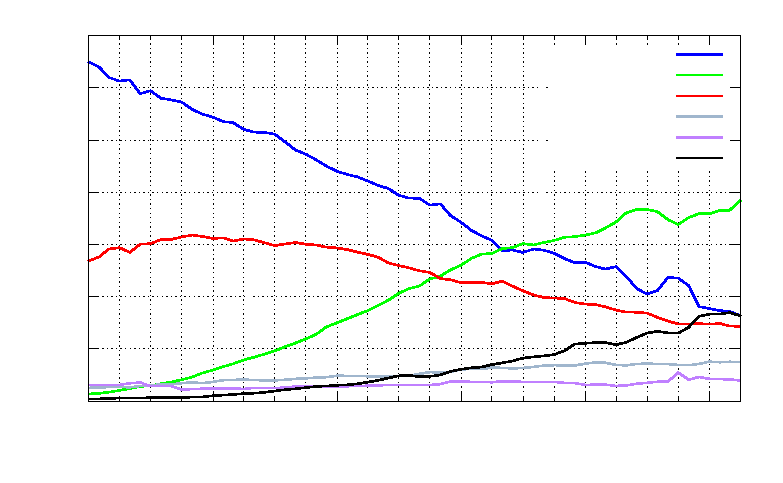
\includegraphics{kap3/figures/browser-ww-monthly-200901-201404-with-mobile}}%
    \gplfronttext
  \end{picture}%
\endgroup

	\caption{Marktanteil von Webbrowsern weltweit \autocite{STATCOUNTER_BROWSERS_09_14}.}
	\label{FIG_BROWSER_MARKETSHARE}
\end{figure}

Deutlich erkennbar ist ein kontinuierlich starker Rückgang des Microsoft Internet Explorers von ehemals 65,0\% zu Anfang des Jahres 2009 auf nur noch 16,4\% im April 2014. Gleichzeitig stieg der Marktanteil von Google Chrome seit dessen Erscheinungsjahr 2008 stetig auf 38,3\% an. Seit 2011 ist Firefoxs Anteil rückläufig und reduzierte sich annähernd um die Hälfte von 26,7\% auf 14,3\%. Während sich Safari auf niedrigem Niveau von 2,6\% auf 7,5\% leicht steigern konnte, weist Operas Kurve nur geringfügige Veränderungen auf. Innerhalb des betrachteten Zeitraums stieg der Anteil hier von 3,1\% auf 4,0\%.
Das Diagramm zeigt zudem eine signifikante Zunahme von mobilen Webbrowsern, die einen klaren Trend hin zur mobilen Nutzung des Webs belegen. So stieg dieser Anteil von 0,4\% stetig auf 16,4\%, was fast einem Sechstel aller Zugriffe entspricht. Eine Erhebung des Statistischen Bundesamts aus dem Jahr 2013 stützt diese These: 2013 nutzten 51\% aller Internetbenutzer im Alter ab 10 Jahren in Deutschland das mobile Internet \autocite{DESTATIS_MOBILE_INTERNET_USERS}.

% anhand - aufgrund
Auf Basis dieser Daten definiert sich die erste Zielvorgabe: Die nähere Überprüfung der Unterstützung der betrachteten 3D-""Technologie innerhalb der fünf meistverwendesten Desktop-Browsern, also Chrome, Internet Explorer, Firefox, Safari und Opera. Je nach Verfügbarkeit der Browser werden diese auf den drei verbreitesten Betriebssystemen, Microsoft Windows, Apple Mac OS X und GNU/Linux getestet.

Aufgrund des wie in Abbildung \ref{FIG_BROWSER_MARKETSHARE} gezeigten, zunehmend stärkeren Einflusses mobiler Geräte stellt deren Untersuchung hinsichtlich dieses Kriteriums ebenso eine Anforderung dar. Betrachtet werden hierbei das hauptsächlich durch Google entwickelte freie Betriebssystem \emph{Android} und Apples mobile Plattform \emph{iOS}.

\subsection{Vermeidung von Browser-Plugins}
Eine weitere Anforderung stellt die Darstellung der 3D-""Szene unter Vermeidung zusätzlicher Browser-Plugins von Drittherstellern dar. In der langjährigen Geschichte von Web3D gab es zahlreiche Plugin-basierte Ansätze, die sich allesamt langfristig nicht behaupten konnten \autocite{Evans201443}.

Sofern eine explizite Aktion seitens des Benutzers, etwa das Installieren eines Browser-Plugins nötig ist, um eine Webseite mit eingebetter 3D-""Grafik zu betrachten, stellt dies eine Einstiegshürde für den Webauftritt dar und kann dessen Benutzerakzeptanz senken. Viele Benutzer stehen Plugins generell eher skeptisch gegenüber, da sie unbekannte Software darstellen, was häufig von Laien als eine potentielle Gefährdung ihres Computers erachtet wird. Zudem sind Plugins oftmals mühsam zu verwalten sind \autocite{Ortiz:2010}.
Das Installieren von Software verlangt zudem eine gewisse Fachkompetenz des Benutzers, die nicht immer gegeben ist. Dies ist in Anwendungsdomänen wie Schulen, Universitäten und Firmen darüber hinaus aufgrund mangelnder Administrationsrechte grundsätzlich nicht möglich.

Veraltete oder wenig verbreitete Browser-Plugins können tatsächlich ein nicht unerhebliches Sicherheitsrisiko innerhalb des Browsers darstellen, da unentdeckte Schwachstellen innerhalb des Plugin-Codes von Angreifern ausgenutzt werden können (\emph{Exploits}) \autocite{Ortiz:2010}. Weiterhin können Browser-Plugins zu Abstürzen der Software führen. Sowohl Google Chrome als auch Mozilla Firefox führen aufgrund dieser möglichen Sicherheits- und Stabilitätsprobleme zahlreiche als unsicher erachtete Plugins erst nach expliziter Autorisierung des Benutzers aus \autocite{CHROME_BLOCKED_PLUGINS} \autocite{FIREFOX_BLOCKED_PLUGINS}.

Aufgrund all dieser Unzulänglichkeiten von Browser-Plugins sind diese als Abhängigkeit einer Web3D-""Anwendung zu vermeiden.

\subsection{Vergleich der Hard"-ware-Anforderungen}
\label{SECTION:HARDWARE_REQUIREMENTS}

Ebenso entscheidend für die Alltagstauglichkeit und Benutzerakzeptanz der 3D-""Applikation ist deren Hard"-ware-""Anforderung und die generelle \emph{Performance} bei der Darstellung. Da letztere in erster Linie von der verfügbaren Grafik-Hardware abhängt, ist eine absolute Bewertung der Leistungsfähigkeit von X3DOM und WebGL schwierig vorzunehmen. Für die Bewertung der zwei Technologien müssen diese einander daher auf demselben Testsystem gegenüber gestellt werden, um vergleichbare Aussagen bezüglich ihrer Performance treffen zu können. In der Evaluation soll diese auf verschiedenen Betriebssystemen und Webbrowsern verglichen werden.

\begin{figure}[!h]
	\centering
	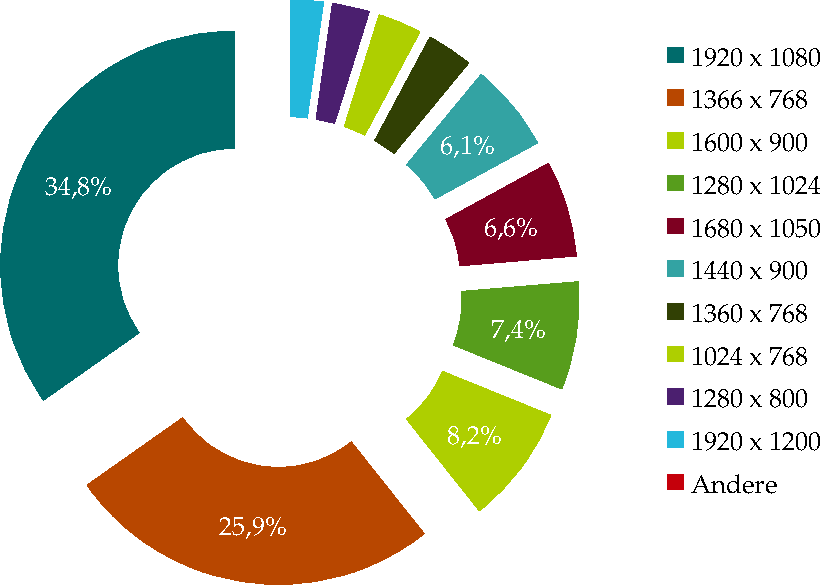
\includegraphics[width=0.5\textwidth]{kap3/figures/hw-top-ten-resolutions-steam-crop.pdf}
	\caption{Zehn meistgenutzte Bildschirmauflösungen auf Steam \autocite{STEAM_HARDWARE_SURVERY}.}
	\label{STEAM_HW_RESOLUTIONS}
\end{figure}

Weiterhin besitzt die Bildschirmauflösung großen Einfluss auf die Hard"-ware-""Anforderung der 3D-""Anwendung, da sich der Berechnungsaufwand während des Renderings durch die höhere Pixelanzahl vergrößert. Abbildung \ref{STEAM_HW_RESOLUTIONS} zeigt die zehn häufigsten Bildschirmauflösungen innerhalb der Spieleplattform Steam des amerikanischen Spieleentwicklers Valve Cooperation im April 2014. Die Statistik entstammt einer nicht repräsentativen monatlich durchgeführten Hard"-ware-Umfrage innerhalb dieses Netzwerks. Die mit Abstand am häufigsten gemessenen Bildschirmauflösungen sind 1920 x 1080 Pixel (\emph{FullHD}) und 1366 x 768 Pixel. Als weiteres Kriterium der Evaluation wird daher die Untersuchung des Einflusses der nachfolgend aufgelisteten fünf Bildschirm-Auflösungen auf die Performance spezifiziert.

\begin{itemize}[noitemsep]
	\item 1024 x 768
    \item 1280 x 1024
	\item 1376 x 768
	\item 1600 x 900
	\item 1920 x 1080
\end{itemize}

\subsection{Import bestehender 3D-""Modelle}

Bei der Umsetzung anspruchsvoller 3D-""Szenen ist die Verwendung von 3D-""Model"-lierungs"-software wie \emph{Blender} \autocite{SOFTWARE_BLENDER}, \emph{3ds Max} \autocite{SOFTWARE_3DS_MAX} oder \emph{Maya} \autocite{SOFTWARE_MAYA} für die Erstellung komplexer Modelle aufgrund der hohen Zahl von Polygonen und komplizierter Texturierungstechniken unabdingbar.
Das einfache und performante Laden solcher im Vorfeld erstellten 3D-Daten ist daher für Anwendungen, die über die Darstellung simpler geometrischer Körper hinausgeht, wesentlich. Um die initiale Ladezeit zu reduzieren, ist das asynchrone Laden von Inhalten von ebenso großer Bedeutung.

Um die Tauglichkeit der verschiedenen Technologien diesbezüglich zu erproben, wird innerhalb der Testumgebung die generelle Unterstützung für das Laden externer 3D-Modelle erprobt.

\subsection{Entwicklungsaufwand}
\label{SEC:DEVELOPMENT_EFFORT}
Ein ebenso zu beachtender Aspekt ist der Aufwand bei der Entwicklung einer Web3D-""Applikation. Ein typischer Webentwickler besitzt Expertenwissen bezüglich der klassischen Websprachen HTML, CSS und JavaScript. Weiterhin kann davon ausgegangen werden, dass er mit mindestens einer der derzeit vorherrschenden serverseitigen Programmiersprachen PHP, Python oder Ruby vertraut ist.
Systemnahe, statisch typisierte Sprachen wie C und C++ können dagegen tendenziell nicht in das Repertoire eines solchen Programmierers gezählt werden. \textcite{Paulson:2007} führt im \emph{Computer Magazine} aus, dass in den letzten Jahren generell ein Trend hin zu dynamischen Sprachen beobachtet werden könne. Hardwarenahe Grafikbibliotheken, die klassischen systemnahen Programmiersprachen wie C ähneln, können daher ein Hindernis bei der Erstellung einer Web3D-Anwendung darstellen.

Ausgehend von diesen Annahmen muss also auch das Vorwissen des Software-""Entwicklers bei der Bewertung der betrachteten 3D-""Techniken mit einfließen. Sofern neue und bis dato unbekannte Konzepte vorliegen, kann dies die Einarbeitungszeit deutlich verlängern und somit die Entwicklungskosten erhöhen.

\section{Anforderungen bezüglich des Nutzungserlebnisses}
% \section{Anforderungen bezüglich der User Experience}

\subsection{Benutzerinteraktion}

Erst durch die Möglichkeit des Benutzers, mit den Objekten innerhalb der 3D-""Welt zu interagieren, kann sich das Potential einer 3D-""Anwendung voll entfalten. Im Gegensatz zu einer statischen, fixen Darstellung von Gegenständen kann durch die benutzergesteuerte Navigation im Raum ein reichhaltigeres, lebendigeres Benutzerelebnis erzielt werden, da der Anwender aktiv Einfluss auf die dargestellte Welt nimmt.

Eine mögliche Navigations-Methode, im Folgenden als Orbit-Navigation bezeichnet, erlaubt das Verschieben, Skalieren und Rotieren von Objekten mit der Maus, wodurch diese aus beliebigen Betrachtungswinkeln untersucht werden können. Darüber hinaus ist eine freie Navigation, in welcher durch die Szenerie \enquote{geflogen} werden kann, gängig. Die Steuerung wird hierbei ebenfalls mit der Maus und zusätzlich der Tastatur realisiert. Die betrachteten 3D-Technologien sollen hinsichtlich dieser und weiterer Navigationsmodelle untersucht werden.

Außerdem soll eine mögliche Umsetzungen für sogenanntes \emph{Picking} betrachtet werden. Picking beschreibt die Auswahl einzelner Objekte im Raum durch den Mauszeiger, um beispielsweise mehr Informationen zu diesem Gegenstand zu erhalten. Durch die dritte Dimension gestaltet sich dieser Prozess dabei weitaus weniger einfach als in einer zweidimensionalen Darstellung, da die Grafikprojektion umgekehrt werden muss.

\subsection{Realistische Grafikdarstellung}

Ein weiterer wichtiger Punkt ist der Grad an Realismus der gezeigten 3D-Szene. Bezugnehmend auf die in Abschnitt \ref{SEC:APPLICATION_DOMAIN} umrissenen Anwendungsfälle sollte beispielsweise die Darstellung eines Produkts in einem Web-Shop möglichst nahe an das reale Vorbild heranreichen. Um eine wirklichkeitsgetreue Darstellung der 3D-Szene zu erzielen, ist insbesondere deren Beleuchtung entscheidend. Dabei ist das ambiente Licht sowie die diffuse und spekulare Reflexion ausschlaggebend. Durch Anwendung aufwendiger Schattierungsverfahren wie Phong-Shading können Materialeigenschaften mit realistischen Reflexionen erzeugt werden. Auch der Schattenwurf ist für ein rundes Gesamtbild der 3D-""Szene wichtig. Die Texturierung der Modelle stellt schließlich eine verhältnismäßig billige Möglichkeit dar, diese realistischer abzubilden.

Globale Beleuchtungsmodelle wie \emph{Raytracing} und \emph{Radiosity} sind in der Lage, nahezu fotorealistische Bilder durch sehr aufwendige Berechnungsverfahren zu erzielen. Aufgrund der hohen Anforderungen an die Hardware und der langen Rechenzeiten sind diese Modelle jedoch für Echtzeit-Grafikdarstellungen im Webbrowser ungeeignet und werden daher nicht näher behandelt.

Um X3DOM und WebGL bezüglich der realistischen Grafikdarstellung zu erproben, wird ein texturiertes 3D-Modell in jeder Technologie mit den ausgeführten Beleuchtungstechniken dargestellt und im Anschluss verglichen.

	\chapter{Betrachtung aktueller 3D-Technologien im Webbrowser}
\label{CHAP:TECHNOLOGIES}

\section{Ursprung von Web3D: Virtual Reality Modeling Language}
Vor der näheren Betrachtung von X3D und WebGL soll zunächst deren Ursprung dargelegt werden, um die grundlegenden Konzepte dieser heutigen Technologien zu erläutern. Die Geschichte von Web3D reicht über zwei Jahrzehnte zurück, in denen es eine Vielzahl von Bestrebungen verschiedenster Institutionen gab, 3D-""Grafik im World Wide Web (WWW) zu etablieren. Die überwiegende Mehrheit dieser Ansätze scheiterte jedoch und konnte nie eine erwähnenswerte Bedeutung im WWW erlangen \autocite{Evans201443}. Erst innerhalb der letzten Jahre entwickelte sich durch das Aufkommen WebGLs eine neue Dynamik innerhalb dieses Felds.

Die ersten Anfänge der webbasierten 3D-""Computergrafik gehen bis ins Frühjahr 1994 zurück, als der Erfinder des noch jungen World Wide Webs, Tim Berners-Lee, öffentlich dazu aufrief eine Spezifikation für virtuelle Realität zu entwickeln \autocite{Parisi:2012}. Der Informatiker Dave Raggett, der seit 1992 an der Entwicklung zahlreicher Web-Standards richtungsweisend beteiligt war \autocite{PEOPLE_OF_THE_W3C_RAGGETT}, reichte daraufhin seine Publikation \enquote{\emph{Extending WWW to support Platform Independent Virtual Reality}} für die im selben Jahr stattfindende erste internationale World Wide Web Konferenz (\emph{WWW1}) in Genf ein. Ragget prägte innerhalb dieser Arbeit den Begriff \emph{Virtual Reality Markup Language} (VRML\footnote{Gesprochen \emph{vermal}.}) und beschrieb seine Vision von webbasierter virtueller Realität  \autocite{VMRL_RAGGETT}: Eine Auszeichnungssprache auf Basis der \emph{Standard Generalized Markup Language} (SGML) soll es ermöglichen, hierarchische 3D-""Szenen auf einer abstrakten Ebene deklarativ zu beschreiben.

Auf der WWW1 im Mai 1994 bildete sich daraufhin auf Initiave von Ragget und Berners-Lee hin die sogenannte VRML BOF\footnote{Eine sogenannte \emph{Birds of a feather} (BOF) stellt eine informelle Diskussionsrunde von Experten zu einem spezifischen Thema dar. Diese finden insbesondere im Umfeld der Internet Engineering Task Force häufig Anwendung \autocite{RFC5434} \autocite{IETF_BOF_PROCEDURES}.}. Ziel dieser Expertenrunde war die Diskussion bereits bestehender Ansätze von 3D-""Visualisierung mit Fokus auf der Interaktion mit dem WWW. Der auf diesem Gebiet Pionierarbeit leistende Ingenieur Mark Pesce stellte hierbei einen in Zusammenarbeit mit dem Softwareentwickler Tony Parisi entwickelten einfachen Prototypen vor \autocite{Parisi:2012}. Die Demonstration zeigte eine einfache, dreidimensionale Darstellung eines Würfels und ermöglichte die Interaktion mit dem WWW, indem eine URL aufgerufen wurde, wenn man auf die Geometrie klickte. Der Grundstein für die weitere Entwicklung der Virtual Reality Modeling Language im Besonderen und der webbasierten Computergrafik im Allgemeinen war somit gelegt. Um den Bezug zur Computergrafik zu verdeutlichen, wurde die Sprache kurz darauf in Virtual Reality \emph{Modeling} Language umbenannt \autocite{VRML_10_SPECIFICATION}.

Die daraufhin gegründete, schnell wachsende Arbeitsgruppe rund um die \emph{www-vrml} Mailing-Liste einigte sich auf das ehrgeizige Ziel, eine erste Spezifikation noch innerhalb des Jahres 1994 fertigzustellen \autocite{VRML_10_SPECIFICATION}. Aufgrund der guten Basis, die das \emph{Inventor Format} des amerikanischen Computerherstellers \emph{Silicon Graphics} bot, entschied man sich für dieses als Ausgangspunkt für die weitere Entwicklung der Sprache. Tatsächlich konnte VRML 1.0 im November vollendet werden.

Zwei Jahre später wurde deren deutlich ausgereiftere Version 2.0 der Spezifikation fertiggestellt und 1997 zu einem ISO-Standard\footnote{ISO/IEC 14772-1:1997.} \autocite{VRML_20_ISO} erhoben. Zur stetigen Weiterentwicklung und Schutz dieser neuen, als \emph{VRML97} bekannt gewordenen, offenen Spezifikation wurde kurze Zeit später das \emph{VRML Consortium} gegründet. Die Non-Profit-Organisation, die inzwischen den Namen \emph{Web3D Consortium} trägt, betreut bis heute die Entwicklung des VRML-Nachfolgers X3D und treibt dessen Verbreitung voran. Sie setzt sich aus Unternehmen, akademischen Institutionen und Einzelpersonen zusammen \autocite{WEB3D_CONSORTIUM_ABOUT}.

Trotz der hohen Erwartungen konnte sich die VRML nie in dem Maße im WWW durchsetzen, wie es sich deren Entwickler zunächst erwartet hatten. Die Gründe hierfür sind vielfältig: Zunächst war die Installation eines Browser-Plugins zwingend notwendig, um das Format innerhalb des Webbrowsers darstellen zu können. Die Hardware des durchschnittligen damaligen Personal Computers wies darüber hinaus in vielen Fällen eine unzureichende Leistung, sodass rechenaufwändige 3D-""Szenerien nicht zu realisieren waren. Weiterhin war die Geschwindigkeit damaliger Internetanschlüsse zu gering, um die relativ großen Datenmengen, die bei Computergrafik typischerweise anfallen, bewältigen zu können.


\section{Extensible 3D und X3DOM}
\subsection{Aufbau von X3D}

Zwei Jahre nach Veröffentlichung des VRML97-Standards begann eine Arbeitsgruppe des Web3D Consortiums 1999 mit der Entwicklung des Nachfolgers von VRML, \emph{Extensible 3D} \autocite{Daly:2007}. Dieser X3D abgekürzte, freie Standard wurde 2004 ebenso wie zuvor VRML zu einem ISO-Standard\footnote{ISO/IEC 19775-1.} \autocite{Brutzman:2007:XEG:1214715}. Bei der Entwicklung X3Ds wurde auf eine Abwärtskompatiblität zu VRML97 geachtet. Das \enquote{\emph{X}} im Namen impliziert bereits die Nutzung der \emph{Extensible Markup Language (XML)} als Grundlage dieses neuen Grafikformats. Hierdurch wurde eine größere Konvergenz zu bestehenden Webtechnologien wie HTML und XHTML erzielt.

X3D nutzt einen gerichteten, azyklischen Szenengraph zur Repräsentation einer 3D-Szene (vgl. Abbildung \ref{FIG:SCENEGRAPH_EXAMPLE}). Knoten unterhalb der Wurzel des Graphen (dem \emph{Universum}) stellen dabei sämtliche Objekte der Welt dar. Die X3D-Spezifikation definiert eine große Zahl von Knoten, welche alle benötigten Elemente einer Grafikdarstellung wie Geometrien, Lichtquellen, Kameras, Texturen, Transformationen et cetera abbilden. Der Szenengraph kann in drei Formaten abgespeichert werden. Zur Verfügung stehen ein XML-Format, die klassische VRML-Notation und schließlich ein komprimiertes Binärformat \autocite{Daly:2007}. Für die Darstellung des Formats ist ein spezieller \emph{X3D-Viewer} notwendig. Dieser erzeugt aus dem X3D-Szenengraph eine 3D-Darstellung, die frei von allen Seiten betrachtet werden kann.

Da die X3D-Spezifikation sehr umfangreich ist, existieren sogenannte \emph{Profile}, welche eine Menge von Knoten für eine bestimmte Anwendungsdomäne bündeln. Hierdurch ist es möglich, nur tatsächlich benötigte Knoten des Standards zu laden.

\subsection{Das Framework X3DOM}

\subsubsection{Entstehung}

Während der Ausarbeitung des neuen HTML5-Standards stellte X3D den vom World Wide Web Consortium favorisierten Standard für die Realisierung von Web3D-Inhalten dar. Der Arbeitsentwurf der HTML5-Spezifikationen aus dem Jahr 2009 vermerkt diesbezüglich:

\begin{itquote}
	\enquote{Embedding 3D imagery into XHTML documents is the domain of X3D, or technologies based on X3D that are namespace-aware.} \autocite{W3C_HTML5_SPEC_WORKING_DRAFT_12_2009}
\end{itquote}

Diese äußerst knappe Formulierung definiert jedoch in keinster Weise näher, wie eine Plugin-freie Integration von X3D in HTML aussehen könnte. Behr et al. vom Fraunhofer Institut für graphische Datenverarbeitung Darmstadt publizierten daraufhin im selben Jahr ihren Ansatz, wie X3D-Inhalte direkt in HTML eingebettet werden könnten \autocite{Behr:2009:XDH:1559764.1559784}. Ziel des vorgeschlagenen Integrations-Modells \emph{X3DOM} ist eine wechselseitige Verknüpfung zwischen bestehenden Webtechnologien wie dem \emph{Document Object Model} und X3D. Die Autoren erhoffen sich, langfristig eine ähnliche Entwicklung anzustoßen, wie sie das Vektorgrafikformat \emph{Scalable Vector Graphics} (SVG) im WWW durchlief \autocite{Behr:2009:XDH:1559764.1559784}. Während SVG zunächst nur in einigen wenigen Browsern unterstützt wurde, ist dieser Standard inzwischen überall nativ implementiert \autocite{CANIUSE_SVG}. Zum Zeitpunkt der Veröffentlichung dieser Arbeit lag X3DOM noch in einer frühen \emph{Pre-Alpha}-Version vor und zahlreiche Details der Implementierung blieben offen.

\subsubsection{Architektur}
\label{SEC:X3D_ARCHITECTURE}

Im darauffolgenden Jahr legten \textcite{Behr:2010:SAH:1836049.1836077} in einer weiteren Arbeit die zuvor abstrakt dargestellten Ideen ihres Modells mittels der inzwischen gereiften Architektur des X3DOM-Frameworks konkret dar. Grundgedanke von X3DOM ist die Bereitstellung einer einheitlichen Schnittstelle zur deklarativen Programmierung von 3D-Szenen. Hierbei werden die direkt innerhalb des HTML-Dokuments eingebetteten X3D-Knoten wechselseitig mit dem X3D-System synchronisiert. Durch das Hinzufügen, Löschen und Abändern dieser DOM-Elemente kann der Anwendungs-Entwickler die 3D-Szene mittels einfacher JavaScript-Aufrufe dynamisch anpassen.
Zusätzlich zu den im X3D-Standard spezifizierten Attributen fügt X3DOM vielen Knoten weitere Eigenschaften hinzu, die deren Benutzung weiter vereinfachen.

\begin{figure}
	\centering
	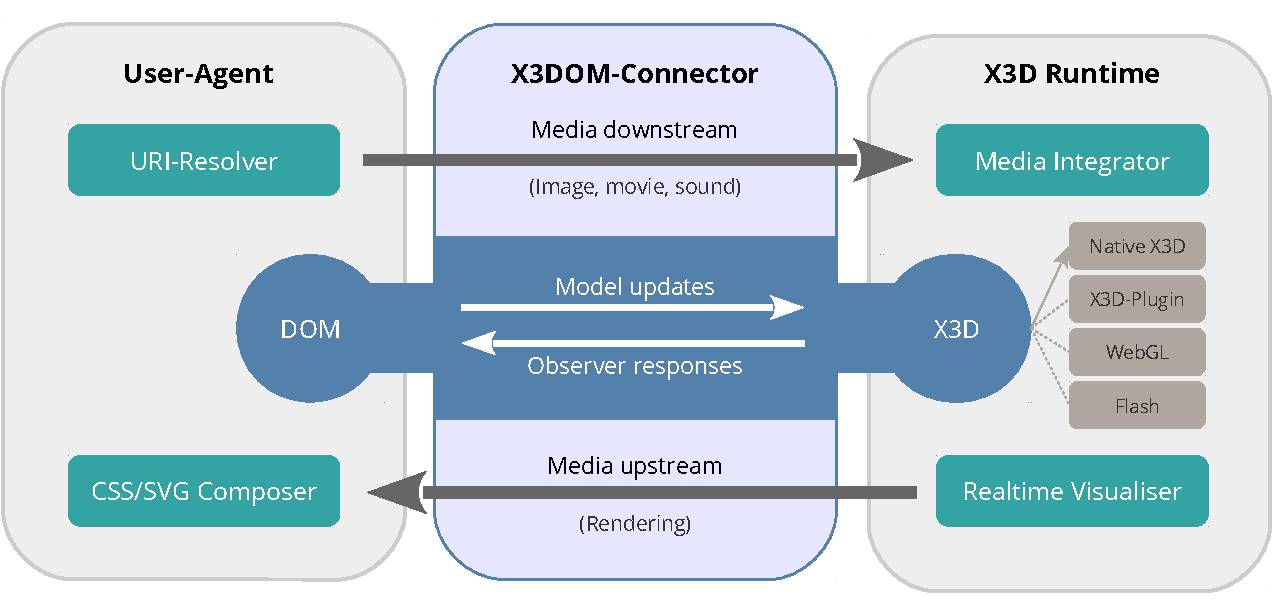
\includegraphics[width=0.9\textwidth]{kap4/x3d/figures/x3dom_architecture-crop.pdf}
	\caption{Architektonischer Aufbau von X3DOM. Geringfügig adaptiert nach \textcite{Behr:2010:SAH:1836049.1836077}.}
	\label{FIG:X3DOM_ARCHITECTURE}
\end{figure}

Die in Abbildung \ref{FIG:X3DOM_ARCHITECTURE} gezeigte Architektur X3DOMs besteht im Wesentlichen aus drei Komponenten: Dem \emph{User Agent}, dem X3DOM-Connector und dem X3D-Runtime.

Ersteres entspricht hier dem Webbrowser. Dieser enthält das Document Object Model und die hierin integrierten X3D-Knoten. Der Browser ermöglicht es weiterhin Multimedia-Dateien wie Grafiken, Video und Audio durch seinen \emph{URI-Resolver} von einem Server herunterzuladen, um diese X3D bereit zu stellen.

Das X3D-Runtime-Objekt auf der andern Seite des Schemas ist für das eigentliche Rendering der Szene und die Verarbeitung von Benutzereingaben verantwortlich. Die Architektur erlaubt hierbei mehrere sogenannter \emph{Backends}. Ein Backend stellt die Technologie dar, mit welcher die computergrafischen Berechnungen vollzogen werden. Mittels eines Fallback-Systems wird das Rendering-Backend anhand einer Priorisierung der Technologien ausgewählt. Hierbei wird zunächst überprüft, ob der der Webbrowser X3D nativ darstellen kann oder ob alternativ ein X3D-Plugin vorhanden ist. Schlägt dies fehl, so wird das Rendering durch WebGL realisiert. Ist auch diese Technik nicht verfügbar, wird auf das proprietäre Flash-Plugin ausgewichen. Wenn dies ebenfalls scheitert, kann keine 3D-Darstellung erfolgen \autocite{Behr:2010:SAH:1836049.1836077}. Die X3D-Runtime-Komponente beinhaltet weiterhin einen sogenannten \emph{Media Integrator}, der die vom User Agent geladenen Medien wie beispielsweise Texturen verarbeitet.

Der \emph{X3DOM Connector} fungiert schließlich als Mittelsmann der zwei obigen Komponenten. Er stellt die Verbindung zwischen den X3D-Knoten im DOM des HTML-Dokuments und dem X3D-System her und synchronisiert diese. Wird das DOM durch JavaScript manipuliert, so wird dies an das Runtime-Objekt propagiert, welches die Szene entsprechend neu rendert und das Bild durch den \emph{Media Upstream} an das HTML-Dokument weiterleitet. Gleichzeitig reagiert das System durch ein \emph{Observer}-Entwurfsmuster auf Benutzereingaben, welche durch JavaScript-Events wie \emph{onClick} abgebildet werden.

\subsection{Beispiel: Rotierende Pyramide}
\label{SEC:X3D_EXAMPLE}

Anhand eines einfachen Beispiels wird im Folgenden der strukturelle Aufbau und einige grundlegenden Konzepte einer X3DOM-basierten Grafikdarstellung aufgezeigt, indem der Quelltext konkret Schritt für Schritt erläutert werden. Das Beispiel und sein Gegenstück in WebGL ist auf der beigefügten CD enthalten.

Die exemplarische Anwendung stellt eine Pyramide dar, welche um die Y-Achse rotiert. Durch eine Auswahlliste kann aus einer perspektivischen oder einer orthogonalen Parallelenprojektion gewählt werden. Abbildung \ref{FIG:X3DOM_EXAMPLE_PROJECTIONS} zeigt diese zwei verschiedenen Ansichten. Die Rotation der Figur kann zudem mittels eines Kontrollkästchens (\emph{Checkbox}) jederzeit pausiert werden.

\begin{figure}[htb]
	\centering
	
\includegraphics[width=0.6\textwidth]{kap4/x3d/figures/example_orthogonal_vs_perspective.png}
	\caption{Orthogonale und perspektivischen Darstellung der Pyramide.}
	\label{FIG:X3DOM_EXAMPLE_PROJECTIONS}
\end{figure}

Eine große Stärke X3Ds im Hinblick auf die Nutzung im Word Wide Web liegt in der großen Nähe zu HTML. Da beide Sprachen Anwendungen der Standard Generalized Markup Language (SGML) sind, ist ihr syntaktischer Aufbau sehr ähnlich. Schlüsselworte in eckigen Klammern, sogenannte \enquote{\emph{Tags}}, dienen der logischen und hierarchischen Strukturierung der Inhalte. Ein Knoten kann zusätzlich durch verschiedene Attribute parametrisiert werden.

\smallskip
\begin{listing}[!h]
\begin{htmlcode}
<head>
	<script src='x3dom.js'></script>
</head>
<body>
	<h1>Konventioneller HTML-Code</h1>
	<X3D width='800px' height='600px'>
		<Scene>
			<!-- Elemente des Szenengraphs -->
		</Scene>
	<X3D>
</body>
\end{htmlcode}
\caption{Einbettung des X3D-Szenengraphs in HTML}
\label{LISTING:X3D_EXAMPLE_EMBEDDING_SCENEGRAPH}
\end{listing}

Nach dem Laden des X3DOM-Quelltexts im Kopfbereich eines HTML-Dokuments kann X3D direkt in dieses eingebunden werden. Listing \ref{LISTING:X3D_EXAMPLE_EMBEDDING_SCENEGRAPH} zeigt diese Einbettung mittels des speziellen X3D-Tags. Durch Angabe der \textit{width}- und \textit{height}-Attribute wird die benötigte Größe der Zeichenfläche spezifiziert. Dem X3D-Tag direkt untergeordnet liegt die Wurzel des Szenengraphen, welche sämtlichen weiteren Knoten der Anwendung enthält. Um die Lesbarkeit der folgenden Ausführungen zu gewährleisten, wurde der komplette Quelltext der Szene in Listing \ref{LISTING:X3D_EXAMPLE} auf der nächsten Seite abgedruckt.

\smallskip
\begin{listing}[p]
\htmlinput[firstline=19, lastline=60, firstnumber=19]{kap4/x3d/example/index.html}
\caption{Gesamter Szenengraph des Beispiels.}
\label{LISTING:X3D_EXAMPLE}
\end{listing}

Das kleine Programm kann im Wesentlichen in drei Schritte gegliedert werden:

\smallskip
\begin{enumerate}[noitemsep]
	\item Festlegen der Ansicht und des Navigationsmodus.
	\item Erstellung und Transformation der Pyramiden-Geometrie.
	\item Animation der Figur.
\end{enumerate}

Zunächst wird die Ansicht der Szene mittels des \textit{Viewpoint}-Elements in den Zeilen 21 bis 23 festgelegt. Der Darstellung können beliebig viele solcher Viewpoints hinzugefügt werden. Durch JavaScript können diese anschließend angesteuert und dynamisch aktiviert werden.
Standardmäßig wird hierbei eine perspektivische Projektion verwendet. Für eine orthogonale Parallelenprojektion steht der \textit{OrthoViewpoint} zur Verfügung.
Das \textit{NavigationInfo}-Element definiert daraufhin das Navigationsmodell der Szene, also die Art und Weise, wie die Darstellung durch den Benutzer interaktiv verändert werden kann. X3DOM bietet hierbei eine Vielzahl verschiedener vorgefertiger Modi \autocite{X3DOM_DOCS_NAVIGATION_INFO_NODE}: Während die Kamera bei manchen Modelle frei bewegt werden kann, sind andere auf die nähere Betrachtung eines einzelnen Objekts zugeschnitten. Im Beispiel ist eine solche Navigation deaktiviert.

3D-Modelle werden in X3D mittels des \textit{Shape}\footnote{Engl. für Form oder Gestalt.}-Knotens umgesetzt. Das Format bietet für zahlreiche geometrische Primitive wie Kugeln, Quader, Zylinder et cetera bereits vordefinierte Elemente, die die Erstellung dieser Basisfiguren sehr einfach gestalten. Listing \ref{LISTING:X3D_SHAPE_NODE} zeigt dies exemplarisch durch Deklaration eines Würfels mittels des \textit{Box}-Tags in Zeile 5. Dem Shape-Knoten ist weiterhin das \textit{Appearance}-Element untergeordnet, welches wiederum einen \textit{Material}-Knoten enthält (vgl. Listing \ref{LISTING:X3D_EXAMPLE}, Zeilen 43 - 45). Dieser legt zahlreiche Attribute hinsichtlich der Beleuchtung des Objekts fest: etwa die Reflexionsintensität des ambienten Lichts, die Farbe diffusen Lichts, den Grad spekularer Glanzeffekte und so weiter fest.

\smallskip
\begin{listing}[!h]
\begin{htmlcode}
<Shape>
	<Appearance>
		<Material diffuseColor='0 0.66 0.66'></Material>
	</Appearance>
	<Box></Box>
</Shape>
\end{htmlcode}
\caption{Erstellung einfacher Primitive durch den Shape-Knoten.}
\label{LISTING:X3D_SHAPE_NODE}
\end{listing}

Sofern das Modell durch kein geometrisches Primitiv dargestellt werden kann, bietet X3D durch das \textit{IndexedFaceSet}-Element einen Mechanismus, wie die topologische Struktur eines 3D-Modells durch explizite Angabe der Vertices und Seiten definiert werden kann. Unter der Topologie wird in diesem Zusammenhang die Nachbarschaftsbeziehung der Knotenpunkte, Kanten und Flächenstücke einer Geometrie verstanden. Der IndexedFaceSet-Knoten befindet sich unmittelbar unterhalb des Shape-Elements.
Die Seiten der Figur werden dabei mittels des \textit{CoordIndex}-Elements spezifziert. Durch Angabe dreier oder mehr Indices, der im Kindknoten \textit{Coordinate} gegebenen Vertices, wird ein entsprechendes Polygon erstellt (Zeile 28 ff.). Die Zahl $-1$ dient dabei als Begrenzungszeichen der verschiedenen Seiten. Zu beachten gilt zudem, dass die Indexierung der Vertices bei $0$ beginnt.
Der so kreierten Pyramide wird mittels des \textit{diffuseColor}-Attributs des Material-Knotens die Farbe Türkis zugeordnet (Zeile 44). Farben werden in X3D durch das RGB-Farbmodell angegeben, wobei $1$ der maximalen Intensität eines Farbkanals entspricht.

Die gesamte Geometrie wird durch ein Transformations-Element umhüllt. Dieses ermöglicht die affine Transformation untergeordneter Elemente. In diesem Fall wird die Pyramide in die negative Y-Richtung translatiert (Zeile 26). Das Attribut \textit{DEF} dient der eindeutigen Bezeichnung des Knotens und wird im finalen Animations-Schritt benötigt.

Animationen werden in X3D durch sogenannte Schlüsselbilder (\emph{Keyframes}) realisiert. Hierbei werden verschiedene diskrete Zustände der Animation durch die Keyframes definiert und die Bewegung anschließend durch lineare Interpolation zwischen diesen Werten erzielt. Innerhalb X3Ds sind hierfür mehrere Komponenten nötig: Zunächst wird ein sogenannter \textit{TimeSensor} definiert, welcher die Interpolation der Werte anstößt und die Länge der Animation durch das Attribut \textit{cycleInterval} festlegt (Zeile 49). Die Schlüsselbilder werden innerhalb eines \textit{Interpolator}-Knotens spezifiziert (Zeile 50 f.). Da die Rotation der Figur verändert werden soll, wird ein \textit{OrientationInterpolator} benötigt. Um eine vollständige Drehung umzusetzen wird das Bogenmaß des Winkel im Intervall von $0$ bis $\pi$ interpoliert.
Um diese zwei Komponenten nun zu verknüpfen, führt X3DOM das Konzept von \textit{Routes} ein. Durch dieses Pipeline-artige Konstrukt kann ein automatischer Datenaustausch zwischen verschiedenen Knoten angestoßen werden, sofern eine bestimmte Bedingung zutrifft (vgl. Zeile 55 ff.). Der Zeitsensor im Beispiel initiiert in regelmäßigen Abständen eine zeitabhängige Neuberechnung des aktuellen Rotationswinkels im \textit{OrientationInterpolator}. Sobald sich der Rotationswinkel entsprechend verändert hat, wird dies an den Transformationsknoten propagiert, welcher nun die Rotation der Pyramide anpasst.

Bei Betrachtung des gesamten Quelltexts des Beispiels in Listing \ref{LISTING:X3D_EXAMPLE} wird die Kompaktheit X3Ds deutlich. Bereits wenige XML-Knoten waren ausreichend, um die gewünschte rotierende Pyramide im Webbrowser darzustellen. Sofern eine manuelle Definition der Geometrie nicht notwendig gewesen wäre, wäre das Programm sogar noch deutlich kürzer ausgefallen. Dies unterstreicht die Vorteile des deklarativen Ansatzes von X3D.

Die eingangs zitierte Nennung X3Ds in der HTML5-Spezifikation ist inzwischen nicht mehr in der aktuellen Revision des Arbeitsentwurfs zu finden. Somit muss X3D nicht mehr zwingend als der offizielle, durch das W3C angestrebte Standard für Web3D betrachtet werden. Mit der Web Graphics Library ist eine starke Alternative für einen solchen offiziell unterstützen Grafikstandards entstanden. Im Folgenden soll dieser näher beleuchtet werden.


\section{Web Graphics Library}
Der Ursprung der Web Graphics Library liegt in der Arbeit des inzwischen bei Mozilla angestellten Software-Entwicklers Vladimir Vukićević. Dieser präsentierte 2006 einen ersten experimentellen Prototypen einer Schnittstelle des HTML5-Canvas-Elements\footnote{Canvas: engl. für \enquote{Leinwand}.} zur Grafikbibliothek OpenGL \autocite{WEBGL_ORIGIN_VUKICEVIC}.
Dieser neue Ansatz sollte die native Darstellung von 3D-Grafik im Webbrowser ermöglichen. Hierin liegt der fundamentale Unterschied und Vorteil WebGLs gegenüber allen vorherigen Web3D-Ansätzen: Durch die direkt in den Browser integrierte Schnittstelle zu OpenGL sind Plugins für die Berechnung von 3D-Grafik nicht länger notwendig.

Sowohl Firefox als auch Opera realisierten ein Jahr nach Vukićevićs Vorstoß frühe, eigenständige Implementierungen dieses Ansatzes innerhalb ihrer Browser \autocite{WEBGL_ORIGIN_VUKICEVIC} \autocite{WEBGL_ORIGIN_OPERA}. Während Mozillas Umsetzung von Canvas-3D eine nahezu direktes \emph{Mapping} von JavaScript zu OpenGL darstellte, war Operas Ansatz etwas abstrahierter, um eine bessere Plattformunterstützung zu erzielen.

Zur Standardisierung dieses neuen Vorstoßes für 3D-""Grafik im Web bildete sich 2009 daraufhin die WebGL-Arbeitsgruppe innerhalb der \textit{Khronos Group}. Zwei Jahre später wurde Version 1.0 der Spezifikation auf Basis von \emph{OpenGL ES 2.0} im Februar 2011 fertig gestellt \autocite{KHRONOS_WEBGL_SPEC_10}. Die Khronos Group ist ein seit 2000 bestehendes internationales Industriekonsortium, welches die Entwicklung zahlreicher lizenzfreier und offener Standards im Multimedia-Bereich vorantreibt \autocite{KHRONOS_GROUP_ABOUT}. Zahlreiche namhafte Organisationen und IT-Unternehmen wie Apple, Google, Mozilla und Opera beteiligen sich seither aktiv bei der Entwicklung von WebGL \autocite{KHRONOS_GROUP_WEBGL}.

\subsection{Grundarchitektur}

% TODO: ZEILENNUMMERN ÜBERPRÜFEN!!!

Um die grundlegende Architektur einer WebGL basierten Webanwendung zu verstehen, werden zu Anfang die beteiligten Technologien und deren Zusammenspiel erörtert. Die schematische Abbildung \ref{FIG:WEBGL_ARCHITECTURE} veranschaulicht die Beziehung der einzelnen Komponenten untereinander:

\begin{figure}[ht]
	\centering
	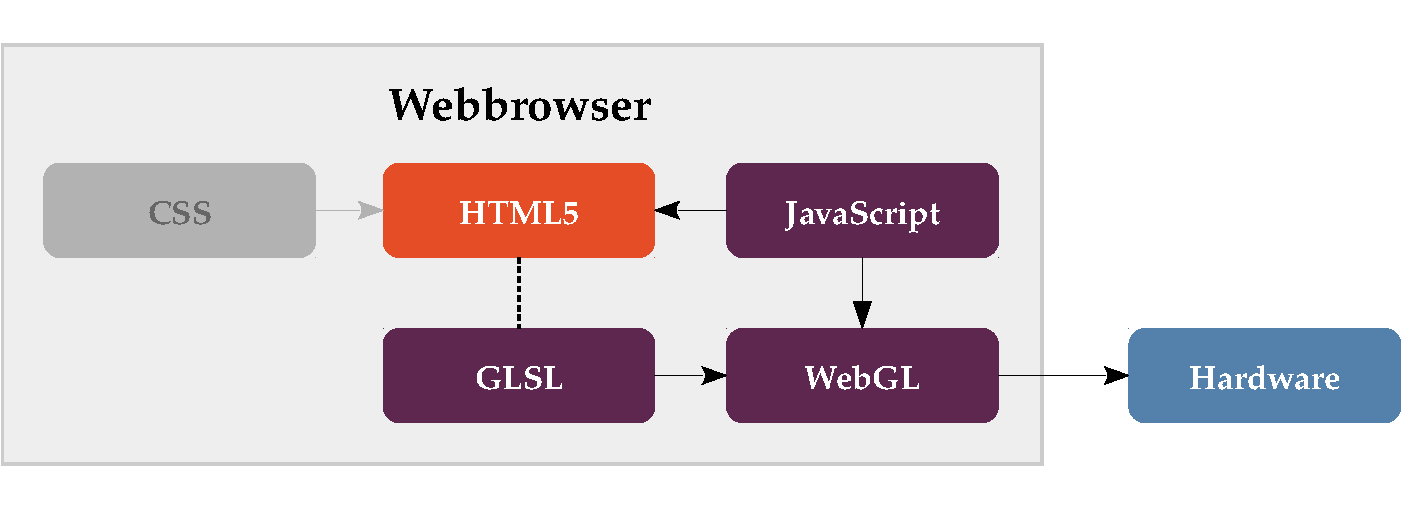
\includegraphics[width=0.8\textwidth]{kap4/webgl/figures/architecture-crop.pdf}
	\caption{Grundarchitektur einer WebGL-basierten Web3D-Anwendung.}
	\label{FIG:WEBGL_ARCHITECTURE}
\end{figure}

Zur Darstellung der 3D-""Grafik ist zunächst ein konventionelles HTML-Dokument nötig. Wichtig ist hierbei eine Deklaration des Dokumentyps als HTML5, da WebGL das erst mit HTML5 eingeführte Canvas-Element benötigt.
Obgleich dieser neue Standard derzeit noch nicht den höchsten Reifegrad einer \emph{W3C Recommendation} erlangt hat, ist dessen Entwicklung weit vorangeschritten. So wurde bereits im Mai 2011 der \enquote{\emph{Last Call}} ausgerufen, also die Aufforderung, letzte Änderungensvorschläge für den Entwurf einzureichen \autocite{W3C_HTML5_LAST_CALL_TARGET_2014}. Weiterhin wurde in selbiger Ankündigung das Jahr 2014 als Zeitpunkt für den Statuswechsel der Spezifikation zu einer W3C-Empfehlung anvisiert.

Das Canvas-Element stellt eine rechteckige Zeichenfläche dar, welche durch JavaScript angesteuert wird und der dynamischen Generierung von Grafiken dient \autocite{W3C_HTML5_SPEC_WORKING_DRAFT}.
Das Element verfügt über mehrere sogenannte \emph{Kontexte}. Ein Kontext stellt die Schnittstelle zu einer Grafik-Implementierung dar und erlaubt es, JavaScript auf der Leinwand zu zeichen. Während der Kontext mit der Bezeichnung \texttt{2d} zweidimensionale Grafiken ermöglicht, kann das Element ebenso als Projektionsfläche dreidimensionaler Grafik dienen. In diesem Fall wird der \emph{WebGLRenderingContext} durch Angabe des Schlüsselworts \texttt{webgl} verwendet. Ein Kontext mit dem Namen \texttt{3d} existiert nicht und liefert kein Ergebnis.

Wie Listing \ref{LISTING:WEBGL_HTML_DOCUMENT} zeigt, besitzt ein HTML-Dokument für die Darstellung von WebGL in seiner minimalen Form einen sehr kompakten Aufbau. Dies verdeutlicht bereits einen paradigmatischen Unterschied zu X3DOM: Die Elemente der 3D-Szene sind nicht Teil von HTML, sondern dieses dient nur der letztendlichen Anzeige der berechneten 3D-Grafik durch das Canvas-Element. Dieses ist mit einem eindeutigen Bezeichner (\emph{ID}) versehen, um es in JavaScript einfach ansprechen zu können (Zeile 8). Weiter sind die Größenangaben der Zeichenfläche für die Initialisierung von WebGL wichtig.
In den Zeilen 9 und 10 wird der Quelltext der Grafikshader innerhalb von Script-Tags eingebunden. Um die Übersichtlichkeit zu wahren, wird deren Inhalt jedoch zunächst ausgelassen. Die Bedeutung und Funktion der Shader wird in Abschnitt \ref{SEC:WEBGL_SHADER} erörtert. Zuletzt wird der ausgelagerte, selbst implementierte WebGL-Code in Zeile 11 geladen (\emph{main.js}).

\smallskip
\begin{listing}[ht]
\begin{htmlcode}
<!DOCTYPE html>
<html>
	<head>
		<meta charset='utf-8'>
		<title>Minimales HTML-Dokument</title>
	</head>
	<body>
		<canvas id='glcanvas' width='800' height='600'></canvas>
		<script id='shader-fs' type='x-shader/x-fragment'></script>
		<script id='shader-vs' type='x-shader/x-vertex'></script>
		<script src='main.js'></script>
	</body>
</html>
\end{htmlcode}
\caption{Aufbau eines minimalen HTML-Dokuments für WebGL.}
\label{LISTING:WEBGL_HTML_DOCUMENT}
\end{listing}

Der nächste Baustein der Architektur JavaScript stellt die zentrale Komponenten des Systems dar. Mittels Abfrage des WebGL-Kontexts durch das Canvas-Elements in HTML wird die Schnittstelle zu WebGL und damit der Grafik-Hardware aufgebaut. Das \emph{Application Programming Interface} (API) der Grafikbibliothek ist durch die Funktionen des Kontext-Objekts abgebildet und ermöglicht so die eigentliche Grafikprogrammmierung. In Abschnitt \ref{SEC:WEBGL_EXAMPLE} werden die konkreten Einzelschritte, die nötig sind, um eine 3D-Darstellung mit WebGL zu erzielen, anhand des Pyramiden-Beispiels erläutert.

Die dritte Komponente der Architektur stellen schließlich die eingangs erwähnten Grafikshader dar. Diese werden im JavaScript-Code eingelesen und innerhalb des WebGL-Systems weiterverarbeitet. Wie die gestrichelte Linie innerhalb des Schemas in Abbildung \ref{FIG:WEBGL_ARCHITECTURE} andeutet, ist der C-ähnliche Shader-Code oftmals innerhalb des HTML-Dokuments eingebettet (vgl. Listing \ref{LISTING:WEBGL_HTML_DOCUMENT}). Grundsätzlich kann dieser Quelltext in einer beliebigen Form als String abgespeichert werden. Er könnte also beispielsweise ebenso aus einer Datenbank stammen. Auch eine direkte Einbettung innerhalb von JavaScripts ist möglich, aber aufgrund der fehlenden Unterstützung der Sprache für mehrzeilige Strings mühsam.

Das letzte Element \emph{Cascading Stylesheets} (CSS) sind keine Notwendigkeit für WebGL per se. Da sie jedoch den De-Facto-Standard für die Gestaltung von Websites und damit auch von Benutzeroberflächen von Webanwendungen darstellen, ist diese Technologie der Vollständigkeit halber ebenso innerhalb des Schemas aufgeführt.

\subsection{Bedeutung und Funktion der Shader}
\label{SEC:WEBGL_SHADER}

Shader sind elementarer Bestandteil heutiger Grafikpipelines und die Ursache derer enormen Flexibilität \autocite[722\psq]{Foley:CG_PRINCIPLES_AND_PRACTICE}. Es handelt sich dabei um kleine Programme, die verschiedenste Effekte beim Rendern von Computergrafik erzielen und direkt innerhalb der \emph{Graphics Processing Unit} auf der Grafikkarte ausgeführt werden. Sie werden in einer eigenen sogenannten Shader-Sprache programmiert. In WebGL wird dabei aufgrund dessen Ursprung auf die \emph{OpenGL ES Shading Language} (GLSL ES) zurückgegriffen.

\begin{itquote}
	\enquote{At the heart of the shading calculations is the simulation of the way light interacts with objects.} -- \textcite{Cook:1984:ST:964965.808602}
\end{itquote}

WebGL kennt zwei Arten von Shadern \autocite{Matsuda:2013}: Den Vertex- und den Fragment-Shader. Ersterer berechnet die letztendliche Position der Vertices im Raum und reicht Vertex-Attribute wie deren Farbe an den Fragment-Shader weiter. Dieser wird innerhalb der Rasterisierungs-Phase der Rendering-Pipeline zu einem späteren Zeitpunkt angewandt.
Der Fragment-Shader dient der Berechnung der Farben der einzelnen Rasterpunkte. Hierfür wird der Einfluss der Lichtquellen auf die Fragmente anhand der verschiedenen Beleuchtungsmodelle und Schattierungsverfahren bestimmt. Ein Fragment beschreibt ein Pixel zusammen mit weiteren Informationen wie der zuhörige Farbe, der Z-Koordinate des Tiefenpuffers und dem Alpha-Wert.

\subsection{Mathematische Bibliotheken}

Bei computergrafischen Berechnungen sind mathematische Vektoren- und Matritzenoperationen aufgrund ihres sehr häufigen Vorkommens von elementarer Bedeutung. Da weder JavaScript innerhalb seiner schmalen Mathematik-""Standardbibliothek noch WebGL, im Gegensatz zu OpenGL ES, eine solche Funktionalität bieten, muss diese durch den Programmierer selbst implementiert werden.

Um diesen immer wiederkehrenden Anforderungen gerecht zu werden, haben sich im WebGL-Umfeld eine Vielzahl von performanten JavaScript-Bibliotheken entwickelt, die diese mathematischen Operationen und Computergrafik-spezifischen Berechnungsroutinen bereitstellen. Im den nachfolgenden Ausführungen wird die populäre Bibliothek \emph{glMatrix} \autocite{SOFTWARE_GL_MATRIX} des Softwareentwicklers Brandon Jones von Google verwendet, um diese Basisfunktionalität zu realisieren.

\subsection{Beispiel: Rotierende Pyramide}
\label{SEC:WEBGL_EXAMPLE}

Analog zu dem in Abschnitt \ref{SEC:X3D_EXAMPLE} gezeigten X3DOM-Beispiel soll im Folgenden die Schritte dargelegt werden, die nötig sind, um die rotierende Pyramide mit WebGL darzustellen. Hierdurch werden die unterschiedlichen paradigmatischen Vorgehensweisen der zwei Ansätze deutlich.

\begin{figure}[!htb]
	\centering
	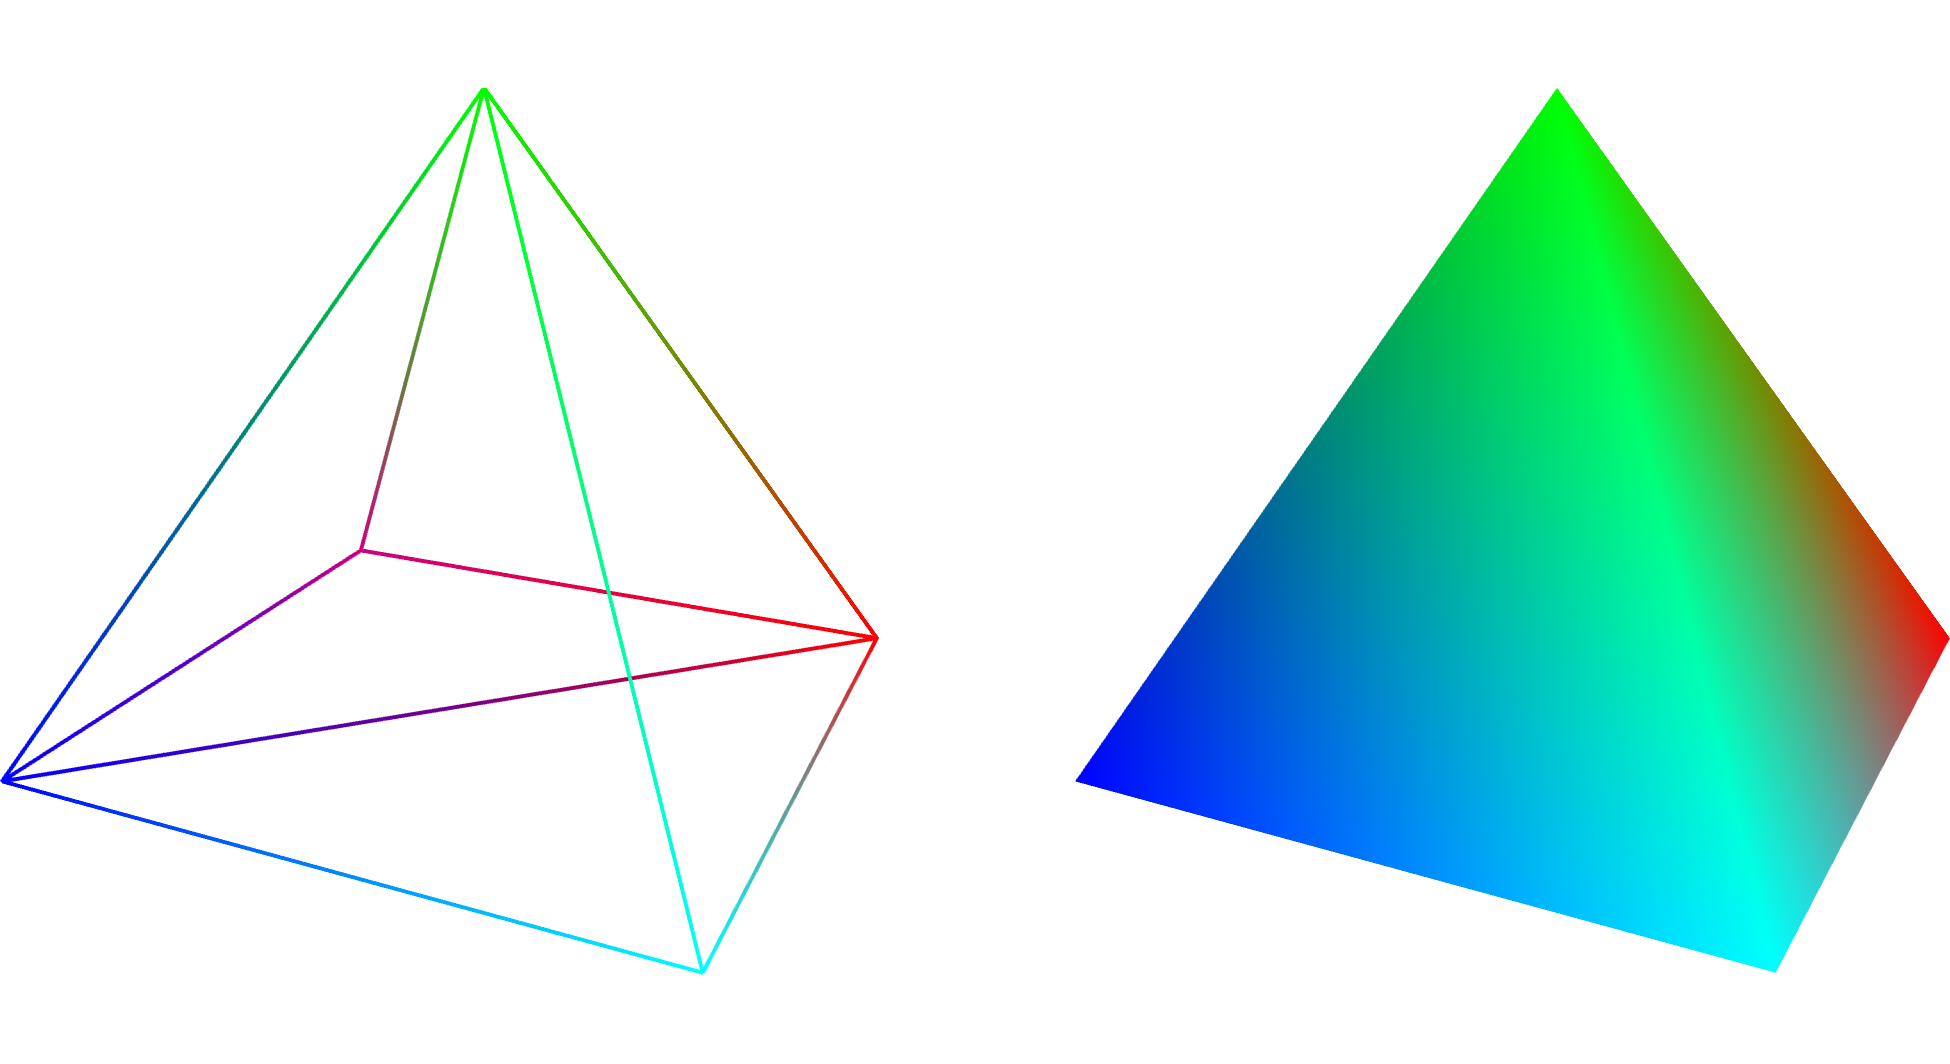
\includegraphics[width=0.6\textwidth]{kap4/webgl/figures/pyramid_views.png}
	\caption{Verschiedene Ansichten der Beispiel-Anwendung.}
	\label{FIG:WEBGL_EXAMPLE_VIEWS}
\end{figure}

Zusätzlich zu den vorherigen Einstellungmöglichkeiten bezüglich Projektionsart und Animation kann die Ansicht nun wie in Abbildung \ref{FIG:WEBGL_EXAMPLE_VIEWS} dargestellt zwischen dem Drahtgittermodell der Figur und gefüllten Flächen umgeschaltet werden.

Der Programmablauf kann wie folgt skizziert werden:

\begin{enumerate}[noitemsep]
	\item Initialisierung des WebGL-Kontexts und Setzen grundlegender Einstellungen.
	\item Erstellung des Fragment- und Vertex-Shaders.
	\item Erstellung der \emph{Buffer Objects} und Schreiben der Vertex-Attribute.
	\item Optional: Animation der geometrischen Figur.
	\item Berechnung und Darstellung des Einzelbilds (Rendering).
\end{enumerate}

Als Einstiegspunkt der Anwendung dient die \texttt{main}-Funktion, welche obigen Ablauf durch mehrere Funktionsaufrufe abbildet. Der Sinn und Zweck der verschiedenen Funktionen wird in den folgenden Abschnitten erklärt.

\smallskip
\begin{listing}[!htb]
\jsginput[firstline=15, lastline=35, firstnumber=15]{kap4/webgl/example/main.js}
\caption{Main-Methode.}
\label{LISTING:WEBGL_EXAMPLE_MAIN}
\end{listing}

\subsubsection{Initialisierung des WebGL-Kontexts}

In den Zeilen 16 bis 25 (vgl. Listing \ref{LISTING:WEBGL_EXAMPLE_MAIN}) wird zunächst der WebGL-Kontext mittels des Canvas-DOM-Elements abgefragt und in der Variable \texttt{gl} gespeichert. In manchen Browser-""Implementierungen von WebGL trägt der Kontext noch die Bezeichnung \texttt{ex"-per"-imen"-tal-""webgl}, welche auf die noch experimentelle Unterstützung der Technologie hinweist. Um eine möglichst breite Browserunterstützung zu erzielen, wird daher auch auf diesen Bezeichner hin geprüft. Die Option \texttt{antialias} aktiviert das Anti-Aliasing und sorgt so für eine glattere Kantendarstellung.

Sofern die Schnittstelle erfolgreich initialisiert werden konnte, werden die weiteren Funktionen \texttt{initGl}, \texttt{initShaders}, \texttt{initBuffers}, und \texttt{tick} aufgerufen. Die \texttt{initGl}-Routine (vgl. Listing \ref{LISTING:WEBGL_EXAMPLE_INIT_GL}) legt einige grundsätzliche Einstellungen fest:
Als erstes wird der Tiefenpuffer aktiviert (\emph{Z-Buffering}). Hierdurch werden Gegenstände, die sich auf der Z-Achse hinter einem weiteren Objekt befinden, im Rasterisierungsschritt verdeckt, so wie es der natürlichen Wahrnehmung entspricht. Weiterhin wird die Breite der zu zeichnenden Linien und die Hintergrundfarbe der Projektionsfläche festgelegt. Der Funktionsaufruf \texttt{gl.clear} in Zeile 50 bewirkt das Zurücksetzen des Farb- und Tiefenpuffers und führt so zu einer komplett weißen, leeren Zeichenfläche.

\smallskip
\begin{listing}[!h]
\jsgginput[firstline=47, lastline=51, firstnumber=47]{kap4/webgl/example/main.js}
\caption{Initialisierung des WebGL-Kontexts.}
\label{LISTING:WEBGL_EXAMPLE_INIT_GL}
\end{listing}

\vspace{1ex}

\begin{listing}[!h]
\jsginput[firstline=62, lastline=75, firstnumber=62]{kap4/webgl/example/main.js}
\caption{Berechnung der Sicht-Projektions-Matrix.}
\label{LISTING:WEBGL_EXAMPLE_CALC_VP_MATRIX}
\end{listing}

Zur Berechnung der Sicht- und Projektionsmatrix wird die Hilfsfunktion \texttt{calc"-View"-Proj"-Matrix} aufgerufen (vgl. Listing \ref{LISTING:WEBGL_EXAMPLE_CALC_VP_MATRIX}). Innerhalb dieser Methode wird zunächst die Sichtmatrix durch Aufruf der \texttt{mat4.lookAt}-Funktion der \emph{glMatrix}"=Bibliothek erstellt. Hierbei fließen Augpunkt, das Zentrum der Beobachtung (\emph{Look-at-Punkt}) und Oben-Vektor ein. Je nach aktueller Einstellung wird anschließend entweder eine orthogonale Projektionsmatrix durch Angabe der Ausdehnung des Sichtvolumens erstellt oder die Projektionsmatrix für eine perspektivische Darstellung erzeugt. In letzerem Fall wird ebenso die Abmessung des \emph{Frustums} und die Distanz der \emph{Front-} und \emph{Backplane} als Parameter benötigt.

Die Berechnung dieses Matrizenprodukts dient der Einsparung von Rechenzeit. Während sich die Modellmatrix durch die Animation kontinuierlich ändert, bleibt die Sicht-Projektions-Matrix größtenteils gleich.

\subsubsection{Initialisierung der Shader}

Im nächsten Schritt werden die im HTML-Dokument eingebetten Shader durch die Hilfsmethode \texttt{getShader} eingelesen und verarbeitet. Hierbei wird je nach Typ ein entsprechendes Shader-Objekt erstellt, der Quelltext aus den Script-Tags eingefügt und dieser schließlich kompiliert. Listing \ref{LISTING:WEBGL_EXAMPLE_GET_SHADER} zeigt den relevanten Abschnitt der Funktion.

\smallskip
\begin{listing}[!htb]
\jsgginput[firstline=110, lastline=120, firstnumber=110,]{kap4/webgl/example/main.js}
\caption{Auslesen der Shader-Quelltexte.}
\label{LISTING:WEBGL_EXAMPLE_GET_SHADER}
\end{listing}

Anschließend wird das Shader-Programm-Objekt erstellt und der kompilierte Shader-Code angehängt. Durch Aufruf der \texttt{linkProgram}"=Methode wird das Programm zu einer für die GPU verarbeitbaren Binärdatei gebunden (\emph{Linking}). Sofern hierbei kein Fehler aufgetreten ist, wird WebGL angewiesen, die so gepackten Shader beim Rendering-Vorgang für die Berechnung der Darstellung zu verwenden (vgl. Listing \ref{LISTING:WEBGL_EXAMPLE_INIT_SHADERS}, Zeile 92). Zuletzt wird die Speicherposition der Uniform-Variable \texttt{uMVPMatrix} innerhalb des Vertex-Shaders abgefragt. Dies ist notwendig, um deren Wert während der späteren Animation aktualisieren zu können. Eine Uniform-Variable zeichnet sich dadurch aus, dass sie sowohl im Vertex- als auch im Fragment-Shader zur Verfügung steht \autocite{Matsuda:2013}.

\smallskip
\begin{listing}[!htb]
\jsginput[firstline=80, lastline=95, firstnumber=80]{kap4/webgl/example/main.js}
\caption{Erstellung und Binden des Shader-Programms.}
\label{LISTING:WEBGL_EXAMPLE_INIT_SHADERS}
\end{listing}

\subsubsection{Erstellung und Schreiben der Daten-Puffer}

Um den Shadern innerhalb von WebGL Daten zu übergeben, werden sogenannte \emph{Vertex Buffer Objects} (VBO) verwendet. Ein solches Buffer Object stellt einen Speicherbereich innerhalb der GPU dar, welcher verschiedene Vertex-Attribute aufnimmt. In der Beispiel-Anwendung beschreiben drei verschiedene solcher Puffer die Geometrie und Farben der Pyramide.
Bei der Definition dieser Rohdaten kommen sogenannte \emph{TypedArrays} zum Einsatz. Diese speziellen Arrays bieten aufgrund ihrer starken Typenbindung bei großen Datenmengen bessere Performance gegenüber konventiellen JavaScript-Feldern, da der Zugriff entsprechend optimiert werden kann \autocite{JS_TYPED_ARRAYS}.

\smallskip
\begin{listing}[!h]
\jsgginput[firstline=134, lastline=149, firstnumber=134]{kap4/webgl/example/main.js}
\caption{Definition der Vertices und Seiten der Pyramide.}
\label{LISTING:WEBGL_EXAMPLE_INIT_BUFFERS_ARRAYS}
\end{listing}

Im ersten Puffer werden die fünf Eckpunkte (\emph{Vertices}) der Figur durch ihre kartesischen Koordinaten im Raum angegeben (vgl. Listing \ref{LISTING:WEBGL_EXAMPLE_INIT_BUFFERS_ARRAYS}). Der zweite Puffer legt die Seiten der Figur fest. Hierfür werden je drei der zuvor definierten Punkte anhand ihrer Indices zu einem Dreieck verbunden. Zu beachten ist, dass die Nummerierung der Indices bei 0 beginnt. Die Reihenfolge der Punkte ist aufgrund des \emph{Backface Culling} wichtig. Dieses Verfahren dient der Verbesserung der Darstellungseffizienz, indem nur die durch den Normalenvektor definierte Vorderseite von Dreiecken gezeichnet wird. Das letzte hier nicht gezeigte Array spezifiziert schließlich die Farben der Pyramide, indem die RGB-Werte den fünf Punkten ihrer Reihenfolge entsprechend zugeordnet werden. Die Farbkanäle werden in WebGL analog zu X3D im Zahlenintervall $[0,1]$ angegeben.

\smallskip
\begin{figure}[!htb]
	\centering
	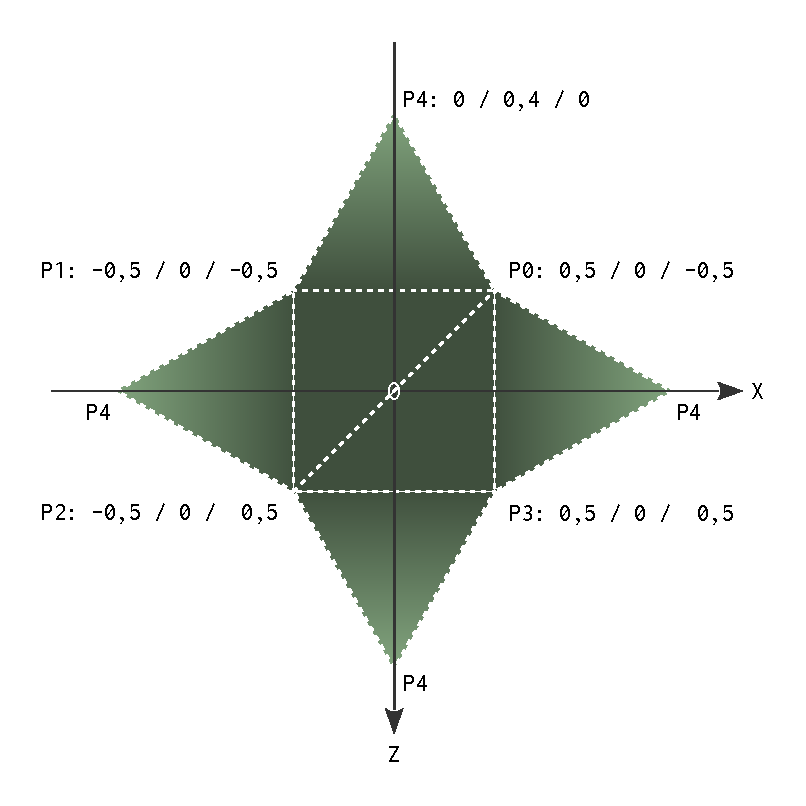
\includegraphics[width=0.5\textwidth]{kap4/webgl/figures/pyramid_sketch-crop.pdf}
	\caption{Topologische Struktur der Pyramide.}
	\label{FIG:WEBGL_EXAMPLE_PYRAMID_SKETCH}
\end{figure}

Abbildung \ref{FIG:WEBGL_EXAMPLE_PYRAMID_SKETCH} veranschaulicht den topologischen Aufbau der Pyramide, indem deren Geometrie innerhalb der XZ-Ebene aufgespannt wurde. Dies erleichtert die Nachvollziehbarkeit der obigen Indices-Zuweisung.

\smallskip
\begin{listing}[!htb]
\begin{minted}[linenos, fontsize=\footnotesize, tabsize=4, baselinestretch=1,firstnumber=168]{javascript}
buffer = gl.createBuffer();
gl.bindBuffer(gl.ARRAY_BUFFER, buffer);
gl.bufferData(gl.ARRAY_BUFFER, vertices, gl.STATIC_DRAW);

FSIZE = vertices.BYTES_PER_ELEMENT;
attribute = gl.getAttribLocation(gl.program, 'aPosition');
gl.vertexAttribPointer(attribute, 3, gl.FLOAT, false, FSIZE * 3, 0);
gl.enableVertexAttribArray(attribute);
\end{minted}
\caption{Schreiben der Puffer-Daten}
\label{LISTING:WEBGL_BINDING_OF_BUFFERS}
\end{listing}

Für das Schreiben der Puffer in den Speicher der GPU sind mehrere Schritte notwendig: Zunächst muss ein Buffer-Objekt durch die WebGL-API erstellt werden. Anschließend wird dieses durch die \texttt{bindBuffer}-Methode als derzeitiger Arbeitspuffer ausgewählt. Die eigentlichen Daten -- hier das Array mit den Vertices -- können dann durch Aufruf von \texttt{bufferData} geschrieben werden (Zeile 168 ff.).
Im nächsten Schritt wird die Speicherposition der Shader-Variable \texttt{aPosition} abgefragt, um diese mit dem Daten-Puffer zu verknüpfen (Zeile 173). Dies wird durch die Funktion \texttt{vertexAttribPointer} realisiert. Dabei gibt deren fünfter Parameter an wie viele Bytes zwischen Beginn und Ende der Definition einer Seite der Pyramide im Vertex-Buffer liegen. Da je drei Eckpunkte eine Seite definieren, wird dieser Wert mit der Länge eines Einzelelements (\texttt{FSIZE}) multipliziert. Mit dem Aufruf von \texttt{enableVertexAttribArray} wird das Vertex-Attribut schließlich aktiviert. Nachdem der Farb- und Indexpuffer auf die selbe Weise an die Grafikhardware gereicht wurden, kann das eigentliche Rendering der Figur beginnen.

\subsubsection{Animation der geometrischen Figur}

Die Funktion \texttt{tick}, welche initial in der \texttt{main}-Routine aufgerufen wurde, ist für die Animation und Berechnung des Einzelbilds verantwortlich. Sofern die Bewegung der Pyramide mittels des Kontrollkästchens aktiviert ist, wird die Animation gestartet (vgl. Listing \ref{LISTING:WEBGL_EXAMPLE_TICK}, Zeile 191). Im Anschluss wird die Rendering-Funktion aufgerufen und die erneute Ausführung von \texttt{tick} durch die \texttt{requestAnimationFrame}-Methode angefordert (Zeile 195 f.).
\texttt{requestAnimationFrame} stellt einen vom Browser bereitgestellte Mechanismus zur Optimierung von JavaScript-Animationen dar \autocite{OPERA_REQUEST_ANIMATION_FRAME}. Der nächste Animationsschritt wird hierbei vom Webbrowser unter Berücksichtigung der aktuellen CPU-Last eingeplant, anstatt diesen nach einem fixen Zeitinkrement auszuführen. Hierdurch wird eine flüssigere Animation erzielt. Ein weiterer Vorteil ist die Einsparung von Rechenzeit und Akkuverbrauch, da die Animationsschleife nur dann ausgeführt wird, wenn der entsprechende Browser-Tab aktiv ist. Dies ist insbesondere bei Mobilgeräten ein wichtiger Aspekt.

\smallskip
\begin{listing}[!htb]
\jsginput[firstline=189, lastline=197, firstnumber=189]{kap4/webgl/example/main.js}
\caption{Einzeliteration der Animation.}
\label{LISTING:WEBGL_EXAMPLE_TICK}
\end{listing}

Die eigentliche Animation der Rotation um die Y-Achse erfolgt durch die Funktion \texttt{animate}. Da das Zeitintervall zwischen zwei Aufrufen der Animations-Methode variieren kann, kann eine ungleichmäßige Bewegung entstehen, sofern stets das gleiche Inkrement zum Rotationswinkel hinzuaddiert wird. Unter Berücksichtigung des Zeitintervalls zwischen zwei Iterationen kann dieses Defizit leicht behoben werden, indem der ermittelte Delta-Wert in die Berechnung dieses Inkrements einfließt (vgl. Listing \ref{LISTING:WEBGL_EXAMPLE_ANIMATE}, Zeile 215). Der Modulo-Operator sichert den Wertebereich von $[0, 360]$ Grad.

\smallskip
\begin{listing}[!htb]
\jsginput[firstline=202, lastline=212, firstnumber=202]{kap4/webgl/example/main.js}
\caption{Animation der Rotation.}
\label{LISTING:WEBGL_EXAMPLE_ANIMATE}
\end{listing}

Da die Grundfläche der Pyramide genau mittig innerhalb der XZ-Ebene liegt und deren Normale auf die Spitze so genau mit der Y-Achse zusammenfällt, ist die Berechnung der Rotation hier sehr einfach. Die Modellmatrix muss lediglich auf die Rotationsmatrix um die Y-Achse für diesen Winkel gesetzt werden. Dies wird durch Aufruf der \texttt{mat4.rotateY}-Funktion aus der \emph{glMatrix}-Bibliothek in Zeile 211 erzielt.

\subsubsection{Rendering des Einzelbilds}

Schließlich kann der Rendering-Prozess der virtuellen Pyramidendarstellung angestoßen werden. Hierfür wird zunächst die MVP-Matrix durch Multiplikation der aktuellen Modellmatrix mit der Sicht-Projektionsmatrix berechnet (vgl. Listing \ref{LISTING:WEBGL_EXAMPLE_RENDER} Zeile 219). Anschließend wird das Ergebnis mittels Aufruf der \texttt{uniformMatrix4fv}-Methode an den Vertex-Shader übergeben.

\smallskip
\begin{listing}[!htb]
\jsginput[firstline=218, lastline=225, firstnumber=218]{kap4/webgl/example/main.js}
\caption{Rendering der Darstellung.}
\label{LISTING:WEBGL_EXAMPLE_RENDER}
\end{listing}

\begin{listing}[!htb]
\begin{jscode}
void main(void) {
	gl_Position = uMVPMatrix * a_Position;
	v_Color = a_Color;
}
\end{jscode}
\caption{Hauptfunktion des Vertex-Shaders.}
\label{LISTING:WEBGL_VERTEX_SHADER}
\end{listing}

Der Vertex-Shader, gezeigt in Listing \ref{LISTING:WEBGL_VERTEX_SHADER}, ist äußerst simpel gehalten und entspricht dem gezeigten Verfahren bei Betrachtung der Standard-Grafikpipeline in Abschnitt \ref{SEC:STANDARD_GRAPHICS_PIPELINE}. Die endgültige Position jedes Vertex wird durch Multiplikation der Koordinaten mit der MVP-Matrix realisiert (vgl. Listing \ref{LISTING:WEBGL_VERTEX_SHADER}, Zeile 3). Der Fragment-Shader ist ebenfalls einfach gehalten. Den einzelnen Fragmenten wird lediglich die zuvor spezifzierte Farbe zugewiesen. Durch die standardmäßige Interpolation der Farben der Eckpunkte bei OpenGL ergeben sich die Farbverläufe auf den Seiten der Figur.

Nachdem der Farb- und der Tiefenpuffer geleert wurde, kann das Bild schließlich mit der gewählten Methode gezeichnet und in den Framebuffer geschrieben werden (vgl. Listing \ref{LISTING:WEBGL_EXAMPLE_RENDER}, Zeile 222 ff.).

\subsection{Three.js als Vertreter eines WebGL-Frameworks}

Wie das vorherige Beispiel zeigt, ist aufgrund des niedrigen Abstraktionsniveaus der WebGL-API im Vergleich zu X3D ein sehr viel höherer Aufwand notwendig, um selbst einfachste dreidimensionale Szenen darzustellen. Da sich jedoch viele Teile des Programmes wie beispielsweise die Abfrage des WebGL-Kontexts oder die Initialisierung der Shader bei jeder WebGL-basierten Anwendung wiederholen, ist eine Generalisierung dieser immer wieder benötigten Funktionalität auf höherer Ebene naheliegend.

Innerhalb der letzten Jahre entstanden so zahlreiche, zum Teil sehr umfangreiche und ausgereifte Frameworks, welche die Umsetzung grafisch anspruchsvoller 3D-""Anwendungen erheblich erleichtern. So können Basiselemente wie Geometrien, Texturen, Lichtquellen, Kameras et cetera mittels weniger Funktionsaufrufe komfortabel erstellt und einem Szenengraph hinzugefügt werden.

Eine Methode zur groben Beurteilung der Popularität von Software stellt die Anzahl von Favorisierungen (Sterne) auf dem Portal \emph{GitHub} dar \autocite{Evans201443}. GitHub ist ein Hosting-Dienst für Repositories der Versionsverwaltung Git, welcher insbesondere bei Open-Source-Projekten beliebt ist. Das Framework \emph{Three.js} des spanischen Webentwicklers Ricardo Cabello\footnote{Besser bekannt als \emph{Mr.doob}.} liegt hierbei mit einem Wert von 15.558 Sternen weit vor dem hinsichtlich dieses Kriteriums zweitpopulärsten Systems \emph{PhiloGL}, welches mit 567 Stimmen lediglich einen Bruchteil dieses Werts verbuchen kann \autocite{SOFTWARE_GITHUB_THREEJS} \autocite{SOFTWARE_GITHUB_PHILOGL}.
Zusätzlich zu der generellen Vereinfachung bei der Erstellung einer 3D-Szene bietet Three.js ähnlich zu X3DOM verschiedene Rendering-Backends, die als Fallback-Lösungen dienen können. Neben WebGL kann die Darstellung auch innerhalb eines 2D-Canvas, durch SVG oder durch CSS3-Transformationen erfolgen. Aufgrund der deutlich schlechteren Performance dieser Techniken und der Fokusierung dieser Arbeit auf WebGL und X3D, werden diese Technologien jedoch nicht näher betrachtet.

Sämtliche weiteren Untersuchungen von WebGL innerhalb des Evaluationsteils werden aufgrund der genannten Vorteile eines abstrahierten WebGL-Frameworks auf Basis von Three.js realisiert.


	\chapter{Evaluation der 3D-Technologien}
\label{CHAP:EVALUATION}

Nachdem das Grundprinzip und die Funktionsweise von WebGL und X3DOM im vorherigen Kapitel ausführlich dargelegt wurden, werden diese im Folgenden anhand der in Kapitel \ref{CHAP:REQUIREMENTS} spezifizierten Kriterien evaluiert.
Hierfür wird zunächst kurz die Testumgebung beschrieben, welche für die Erprobung der Technologien implementiert wurde, und die verwendete Methodik erläutert. Schließlich wird die eigentliche Evaluation mittels verschiedener Tests durchgeführt und die Ergebnisse im Bezug auf die Zielsetzung bewertet.

\section{Architektur der Testumgebung}

\begin{figure}[htb]
	\centering
	\subfloat[Laden eines 3D-Modells]{
		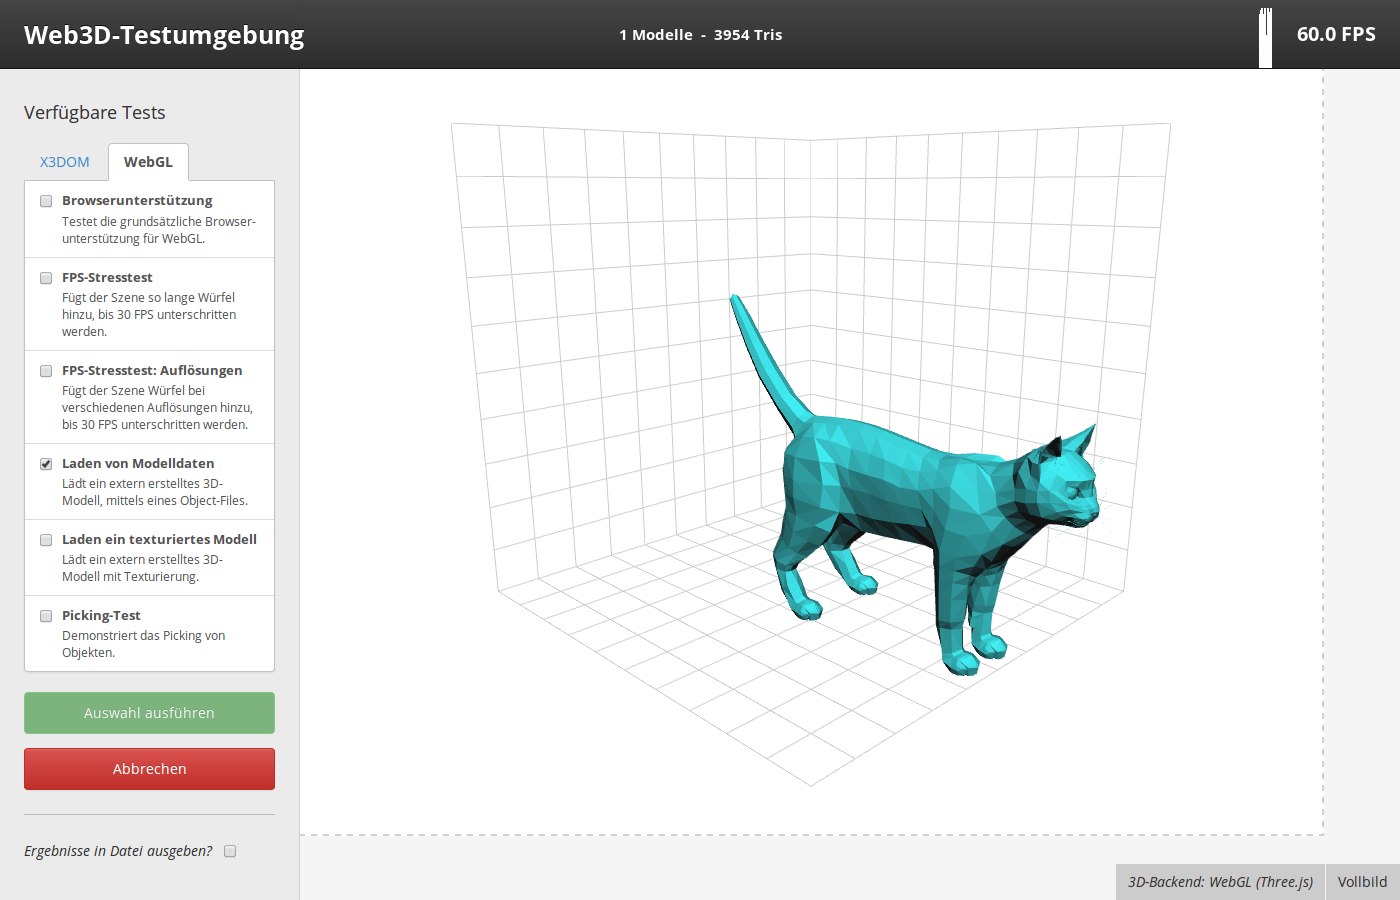
\includegraphics[width=0.48\textwidth]{kap5/figures/test-env-in-action-1.png}
		\label{FIG:WEB3D_TEST_ENV_LOAD_3D_MODEL}
	}
	\hfill
	\subfloat[FPS-Stresstest]{
		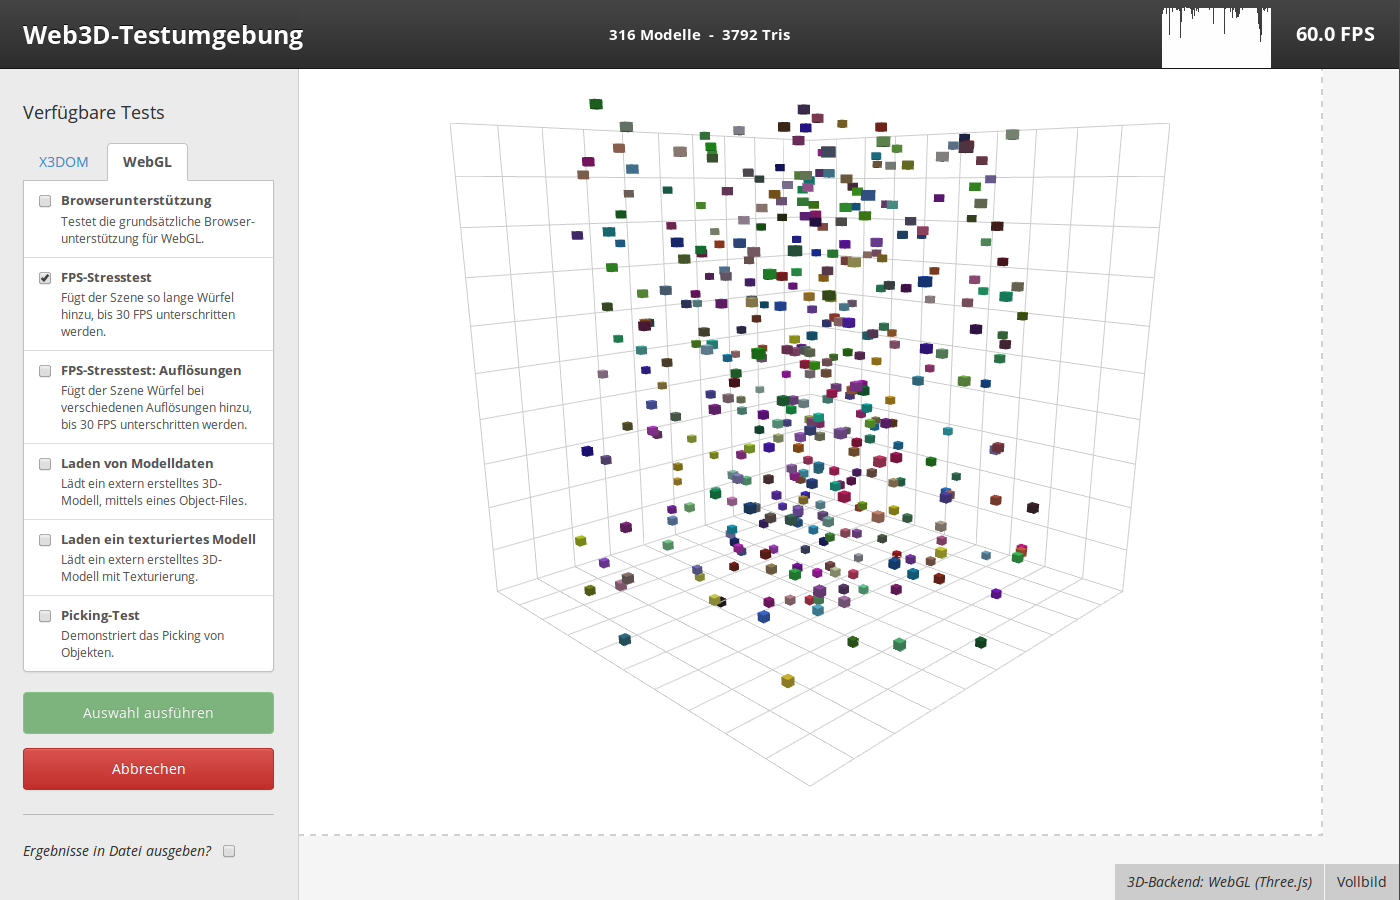
\includegraphics[width=0.48\textwidth]{kap5/figures/test-env-in-action-2.png}
		\label{FIG:WEB3D_TEST_ENV_FPS_STRESSTEST}
	}
	\caption{Verschiedene Tests innerhalb der Testumgebung.}
	\label{FIG:WEB3D_TEST_ENV}
\end{figure}

Zur automatisierten Erprobung von X3DOM und WebGL wurde eine webbasierte Testumgebung umgesetzt, welche die sequentielle Ausführung verschiedener Tests ermöglicht. Die Tests sind auf die spezifizierten Anforderungen zugeschnitten und erproben unterschiedliche Funktionalitäten des Webbrowsers beziehungsweise des Grafiksystems. Abbildung \ref{FIG:TEST_ENV_ARCHITECTURE} zeigt den architektonischen Grundaufbau der Umgebung, die im Folgenden kurz erläutert werden soll.

\begin{figure}[!h]
	\centering
	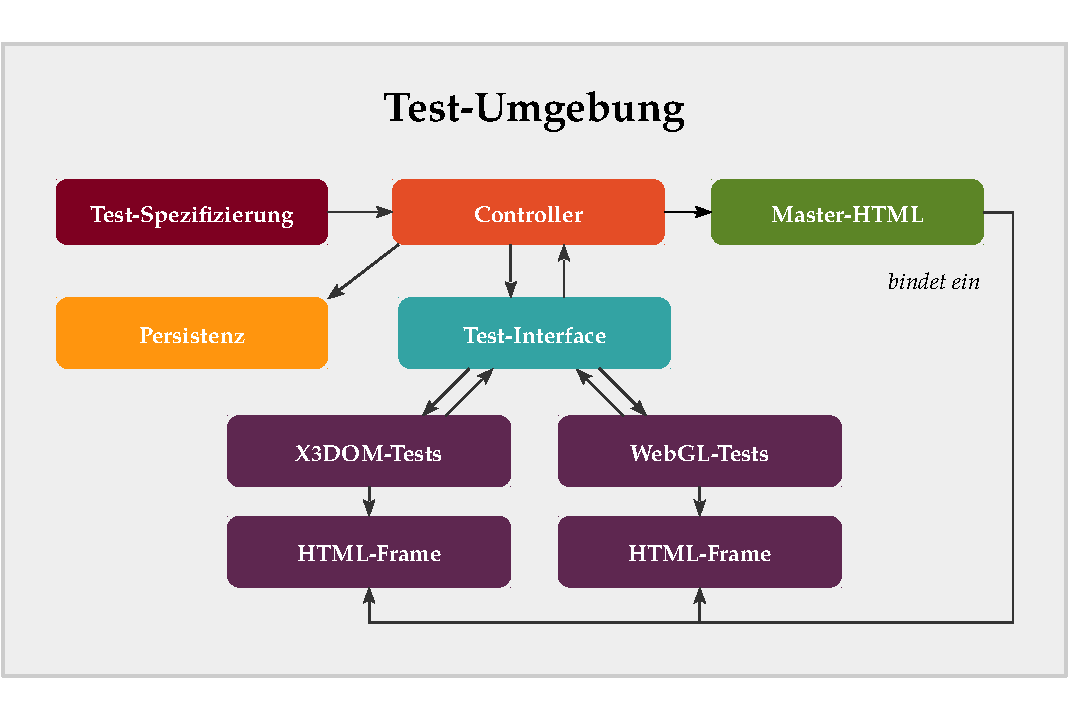
\includegraphics[width=0.8\textwidth]{kap5/figures/test-env-architecture-crop.pdf}
	\caption{Architektur der Testumgebung.}
	\label{FIG:TEST_ENV_ARCHITECTURE}
\end{figure}

Als zentrales Bindeglied der Applikation koordiniert der \emph{Controller} jederzeit den Programmablauf und vermittelt zwischen den einzelnen Komponenten.
Zu Beginn des Ablaufs wird die Test-Spezifikation eingelesen. Diese liegt in Form eines \emph{JSON}-Objekts vor und hat mehrere Funktionen: Zum einen enthält sie die Metadaten der Tests  wie deren textuelle Beschreibung, und zum anderen werden die verschiedenen Testfälle mit einer zugehörigen Funktion verknüpft. Weiterhin werden hier die variierenden Parameter für den späteren Aufruf dieser Methode definiert.

Zur Darstellung der aktuell betrachteten 3D-Technologie dient ein sogenannter \emph{iFrame}. Dieses HTML-""Element ermöglicht das Einbetten eines externen HTML-Dokuments innerhalb eines rechteckigen Rahmens auf einer Webseite. Die so geladene HTML-Seite besitzt ein eigenes \emph{Document Object Model} und operiert größtenteils unabhängig zum Eltern-Dokument. Diese Abschottung hat den Vorteil, dass die 3D-Darstellung innerhalb des \emph{iFrames} in seiner Ausführung durch die Benutzeroberfläche der Testumgebung nicht gestört wird. Darüber hinaus kann das angezeigte HTML-Dokument jederzeit dynamisch durch den Controller mit einem anderen ausgetauscht werden. Dies erleichtert das Testen sowohl von X3D als auch von WebGL in jeweils eigenen Dateien.

Auch die Ausführung der Tests wird vom Controller überwacht. Dieser baut nach der Auswahl der auszuführenden Tests durch den Benutzer eine entsprechende Warteschlange auf und führt die Tests der Reihe nach aus.
Diese sind gegen ein abstrahiertes Test-Interface programmiert und somit unabhängig von ihrer konkreten Implementierung. Für jede der Technologien existiert ein klassenähnliches JavaScript-Objekt, das alle abstrakten Methoden des Test-Interface auf das entsprechende 3D-Framework zugeschnitten, realisiert. Auch das eigentliche Rendern der Szene wird hier umgesetzt.

Um die Messergebnisse der Tests schließlich dauerhaft zu speichern, interagiert der Controller nach Abschluss aller Tests mit der Persistenz-Komponente. Diese dient der Speicherung der volatilen JavaScript-Arrays in einer JSON-Datei, welche daraufhin heruntergeladen werden kann.

\section{Methodik und Testdurchführung}

\subsection{Browserunterstützung und Plattformunabhängigkeit}

Durch das in Abschnitt \ref{SEC:X3D_ARCHITECTURE} beschriebene Fallback-Systems X3DOMs ist ein Test der Browserunterstützung für diese Technologie sehr einfach zu realisieren. Mit dem sogenannten Runtime-Objekt stellt X3DOM eine Schnittstelle zur dynamischen Ansteuerung des Systems bereit. Die Funktion \texttt{backendName} der API liefert den Namen des verwendeten Backends. Falls das Runtime-Objekt nicht existiert, kann X3DOM nicht initialisiert werden, weil keinerlei 3D-Backend zur Verfügung steht. In diesem Fall ist eine 3D-Darstellung durch X3DOM nicht möglich.

\smallskip
\begin{listing}[!htb]
\jsgginput[firstline=146, lastline=150, firstnumber=146]{web3d/tests/x3dom/frame.js}
\caption{Browser-Support-Test für X3DOM.}
\label{LISTING:EVAL_BROWSER_SUPPORT_X3DOM}
\end{listing}

Auch die Überprüfung WebGLs ist leicht zu realisieren. Zunächst wird innerhalb von JavaScript das \texttt{window}-Objekt betrachtet. Dieses stellt das Fenster des Browsers dar und beinhaltet zusätzlich zu dessen Eigenschaften zahlreiche globale Variablen und Schnittstellen zu JavaScript-basierten Webtechnologien. Es wird überprüft, ob \texttt{window} das \texttt{WebGLRenderingContext}-Objekt enthält (vgl. Listing \ref{LISTING:EVAL_BROWSER_SUPPORT_WEBG}, Zeile 170 f.). Wenn dieses Element nicht existiert, ist WebGL in diesem Browser nicht implementiert und es besteht keinerlei Unterstützung für die Technologie. Andernfalls wird versucht den WebGL-Kontext mittels eines dynamisch erstellten Canvas-Elements auszulesen (Zeile 173 ff.). Falls dies fehlschlägt, so ist anzunehmen dass der Webbrowser zwar eine grundsätzliche Unterstützung für WebGL besitzt, aber die Technologie Browser-intern deaktiviert ist.

\smallskip
\begin{listing}[!htb]
\jsgginput[firstline=208, lastline=222, firstnumber=208]{web3d/tests/webgl/frame.js}
\caption{Browser-Support-Test für WebGL.}
\label{LISTING:EVAL_BROWSER_SUPPORT_WEBG}
\end{listing}

Ursache hierfür kann ein instabiler Grafiktreiber beziehungsweise zu schwache Hardware sein. Der Browser unterbindet die Ausführung von WebGL dann anhand einer durch den Hersteller verwalteten \emph{Blacklist}. Die Blacklist beinhaltet Hardwarekomponenten, die dafür bekannt sind, Probleme zu verursachen. Viele Browser erlauben jedoch das explizite Überschreiben dieser internen Deaktivierung WebGLs durch das Setzen sogenannter \emph{Flags} in speziellen Einstellungsdialogen. In Chrome steht dieser beispielsweise bei Eingabe der Adresse \enquote{\texttt{about:flags}} zur Verfügung. In einigen Browser-Versionen ist WebGL darüber hinaus standardmäßig deaktiviert, da die Technologie durch den Hersteller als noch zu experimentell erachtet wird.

Tabelle \ref{TAB_BROWSER_SUPPORT} auf der nächsten Seite zeigt die Testergebnisse dieser Überprüfung auf den betrachteten Plattformen. Wie in der Anforderungsanalyse spezifiziert, wurden hierbei die gängigen Desktop-Betriebsysteme (Windows, Mac OS X und GNU/Linux) untersucht. Weiterhin wurde die Unterstützung innerhalb der mobilen Plattformen Android 4.4 und der aktuellen und zukünftigen Version von iOS getestet (Version 7 und 8).

\begin{table}[tbp]
	\centering
	\small
	\begin{tabularx}{\textwidth}{llYYYYYYY}
		\toprule
						& Gerät
						& \footnotesize 
\includegraphics[height=1em]{kap5/figures/chrome.eps}\hspace{1ex}\textsf{36}
						& \footnotesize 
\includegraphics[height=1em]{kap5/figures/firefox.eps}\hspace{1ex}\textsf{31}
						& \footnotesize 
\includegraphics[height=1em]{kap5/figures/ie.eps}\hspace{1ex}\textsf{9}
						& \footnotesize 
\includegraphics[height=1em]{kap5/figures/ie.eps}\hspace{1ex}\textsf{10}
						& \footnotesize 
\includegraphics[height=1em]{kap5/figures/ie.eps}\hspace{1ex}\textsf{11}
						& \footnotesize 
\includegraphics[height=1em]{kap5/figures/opera.eps}\hspace{1ex}\textsf{23}\textsuperscript{*}
						& \footnotesize 
\includegraphics[height=1em]{kap5/figures/safari.eps}\hspace{1ex}\textsf{7} \\
		\midrule
		\small
		Windows 7		& Desktop
						& \xpie{2} \wpie{1}
						& \xpie{2} \wpie{1}
						& \xpie{1} \wpie{0}
						& \xpie{1} \wpie{0}
						& \xpie{2} \wpie{1}
						& \xpie{2} \wpie{1}
						& - 					\\
		Mac OS X 10.9	& Notebook % DONE
						& \xpie{2} \wpie{1}
						& \xpie{2} \wpie{1}
						& --
						& --
						& --
						& \xpie{2} \wpie{1}
						& \xpie{1} \wpie{0}	 	\\
		Ubuntu 14.04	& Desktop
						& \xpie{2} \wpie{1}
						& \xpie{2} \wpie{1}
						& --
						& --
						& --
						& \xpie{2} \wpie{0.5}
						& -- 					\\
		Arch Linux		& Desktop %DONE
						& \xpie{2} \wpie{1}
						& \xpie{2} \wpie{1}
						& --
						& --
						& --
						& \xpie{2} \wpie{0.5}
						& -- 					\\
		Android 4.4 	& Nexus 7 % DONE
						& \xpie{2} \wpie{1}
						& \xpie{2} \wpie{1}
						& --
						& --
						& --
						& \xpie{2} \wpie{1}
						& --          			\\
		iOS 7			& iPad 3 % DONE
						& \xpie{0} \wpie{0}
						& --
						& --
						& --
						& --
						& --
						& \xpie{0} \wpie{0} 	\\
		iOS 8 (\emph{Beta})	& Simulator % DONE
						& \xpie{2} \wpie{1}
						& --
						& --
						& --
						& --
						& --
						& \xpie{2} \wpie{1} 	\\
		Android 4.4 	& Nexus 5 % DONE
						& \xpie{2} \wpie{1}
						& \xpie{2} \wpie{1}
						& --
						& --
						& --
						& \xpie{2} \wpie{1}
						& --          			\\
		iOS 7			& iPhone 5s
						& \xpie{0} \wpie{0}
						& --
						& --
						& --
						& --
						& --
						& \xpie{0} \wpie{0}		\\
		\bottomrule
	\end{tabularx}
	\begin{minipage}{0.25\linewidth}%
		\vspace{1ex}
		\begin{itemize}[leftmargin=*,label={}]
			\scriptsize
			\itemsep0em
			\item\tikz \fill [x3domc] (0.1,0.1) rectangle (0.25,0.25);\hspace{1.5ex}X3DOM
			\item\tikz \fill [webglc] (0.1,0.1) rectangle (0.25,0.25);\hspace{1.5ex}WebGL
			\item\small--\scriptsize\hspace{1.5ex}Browser nicht verfügbar
		\end{itemize}
	\end{minipage}%
	\begin{minipage}{0.25\linewidth}%
		\vspace{1ex}
		\begin{itemize}[leftmargin=*,label={}]
			\scriptsize
			\itemsep0em
			\item\small\xpie{0}\scriptsize\hspace{1.5ex}Keine Unterstützung
			\item\small\xpie{1}\scriptsize\hspace{1.5ex}Flash-Backend
			\item\small\xpie{2}\scriptsize\hspace{1.5ex}WebGL-Backend
		\end{itemize}
	\end{minipage}%
	\begin{minipage}{0.25\linewidth}%
		\vspace{1ex}
		\begin{itemize}[label={}]
			\scriptsize
			\itemsep0em
			\item\small\xpie{3}\scriptsize\hspace{1.5ex}X3D-Plugin
			\item\small\xpie{4}\scriptsize\hspace{1.5ex}Natives X3D
			\item%
		\end{itemize}
	\end{minipage}%
	\begin{minipage}{0.25\linewidth}%
		\vspace{1ex}
		\begin{itemize}[leftmargin=*,label={}]
			\scriptsize
			\itemsep0em
			\item\small\wpie{0}\scriptsize\hspace{1.5ex}Keine Unterstützung
			\item\small\wpie{0.5}\scriptsize\hspace{1.5ex}Teilweise unterstützt
			\item\small\wpie{1}\scriptsize\hspace{1.5ex}Unterstützt
		\end{itemize}
	\end{minipage}%
	\vspace{0.5ex}%
	\center\scriptsize * Anmerkung: Opera unter GNU/Linux in Version 12.
	\vspace{0.5ex}%
	\caption{Unterstützung von X3DOM und WebGL auf verschiedenen Testsystemen.}
	\label{TAB_BROWSER_SUPPORT}
\end{table}

In den meisten Testfällen zeigt sich ein einheitliches Bild: WebGL wird auf fast allen Plattformen nativ unterstützt. Dadurch ist eine Darstellung von X3D durch X3DOM mit entsprechendem Backend möglich. Eine Ausnahme stellt die derzeitige Version 7 von iOS dar: Der Standard-Browser Safari von Apple bietet weder für X3DOM noch für WebGL eine Unterstützung. Aufgrund der fehlenden Unterstützung von iOS für Adobe Flash steht auch dieses Fallback-Model nicht zur Verfügung.
Interessanterweise besteht bereits seit iOS 5 eine Implementierung WebGLs in Safari. Diese ist jedoch abgesehen von der Werbeplattform \emph{iAd} deaktiviert und kann nicht angesprochen werden \autocite{Benin:2012:THM:2338714.2338734}. Wie bereits im Motivationsteil erwähnt, wird mit der Veröffentlichung von iOS 8 jedoch auch dieses Hinderniss durch die Aktivierung WebGLs überwunden sein \autocite{APPLE_WWDC_2014_WEBGL}.
Auch in der Desktop-Variante von Safari unter Mac OS X ist WebGL bis dato nicht verfügbar. Es ist jedoch davon auszugehen, dass WebGL ähnlich zu iOS mit der für Herbst 2014 angesetzten Version 8 von Safari aktiviert sein wird. Sofern das Flash-Plugin installiert ist, bietet der Browser derzeit zumindest eine X3DOM-Unterstützung durch das Flash-Backend.

Ebenso aus dem Raster fallen die Linux-Vertreter Ubuntu 14.04 und Arch Linux. Unter GNU/Linux liegt Opera noch in Version 12 vor und hinkt der aktuellen Versionsnummer 23 nach. Die Ursache für diesen Unterschied ist die 2013 vollzogenen Umstrukturierung des Browsers. Nach einem Wechsel zur HTML-Rendering-Engine \emph{Blink}, einer Abspaltung von \emph{Webkit}, wurde Opera auf Basis von Chromium\footnote{Chromium ist das Open-Source-Projekt hinter Googles Webbrowser Chrome.} neu aufgesetzt \autocite{OPERA_SWITCHES_TO_WEBKIT}. Zwar existiert in Opera 12 eine WebGL-Implementierung, sie ist jedoch standardmäßig deaktiviert und muss durch die oben beschriebene \emph{Flag} im Browser explizit aktiviert werden.

Da WebGL erst ab Internet Explorer 11 unterstützt wird, steht in den Versionen 9 und 10 lediglich bei X3DOM eine Unterstützung für 3D-Darstellung zu Verfügung, wenn ein Flash-Plugin installiert ist.

\subsection{Vergleich der Hardware-Anforderungen}

Um die Hardware-Anforderungen und die Performance der zwei Technologien gegenüberzustellen, wurde innerhalb der Testumgebung ein GPU-Stress-Test implementiert. Hierbei werden der 3D-""Szene so lange Würfel hinzugefügt, bis die Bildwiederholrate (\emph{Framerate}) wie in Abschnitt \ref{SECTION:HARDWARE_REQUIREMENTS} spezifiziert unter 25 Bilder pro Sekunde (\emph{FPS}) fällt. Die Zahl der grafischen Primitive und der Polygone (Dreiecke) wird dabei mit aufgezeichnet. Um eine Vergleichbarkeit der Betriebsysteme zu gewährleisten, wurde der Test auf allen Plattformen in Google Chrome ausgeführt.

\begin{figure}[p]
	\centering
	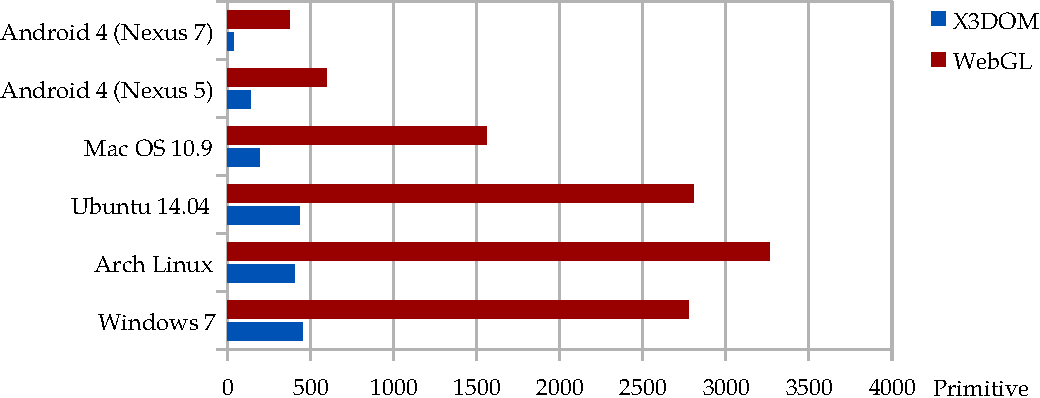
\includegraphics[width=0.9\textwidth]{kap5/figures/test-fps-all-os-chrome-crop.pdf}
	\vspace{0.75ex}
	\caption{FPS-Stresstest für 25 FPS in Google Chrome.}
	\label{FIG:GEOMETRY_TEST_CHROME}
\end{figure}

\begin{figure}[p]
	\centering
	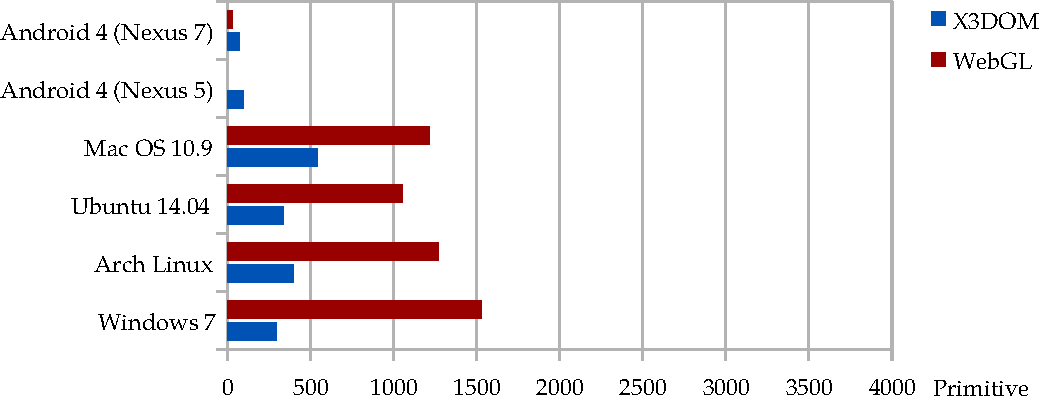
\includegraphics[width=0.9\textwidth]{kap5/figures/test-fps-all-os-ff-crop.pdf}
	\vspace{0.75ex}
	\caption{FPS-Stresstest für 25 FPS in Firefox.}
	\label{FIG:GEOMETRY_TEST_FIREFOXL}
\end{figure}

\begin{figure}[p]
	\centering
	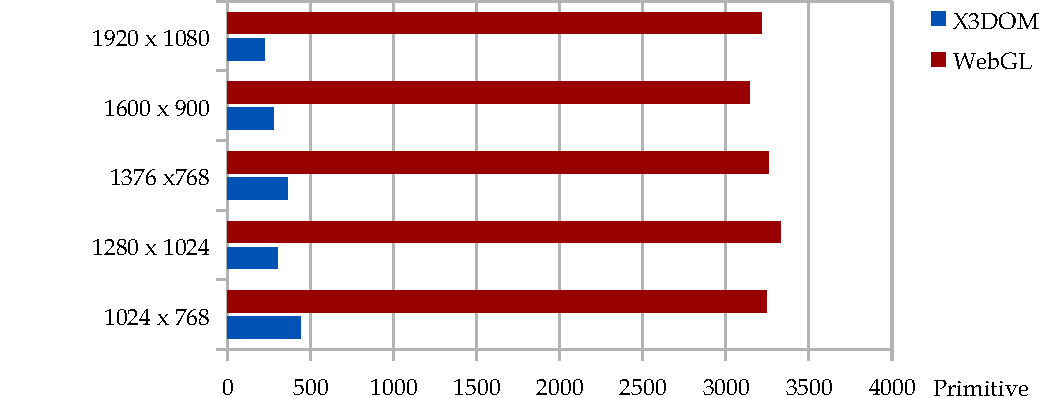
\includegraphics[width=0.9\textwidth]{kap5/figures/test-fps-all-res-chrome-crop.pdf}
	\vspace{0.75ex}
	\caption{FPS-Stresstest für verschiedene Auflösungen.}
	\label{FIG:GEOMETRY_RESOLUTION_TEST_CHROME}
\end{figure}

Die Messergebnisse in Abbildung \ref{FIG:GEOMETRY_TEST_CHROME} auf der nächsten Seite zeigen eine enorme Differenz zwischen X3DOM und WebGL auf. WebGL schafft im Test unter Chrome auf jeder Plattform im Schnitt über sieben mal mehr Primitive als X3DOM darzustellen, ehe die Framerate unter 25 Bilder pro Sekunde fällt.

Da X3DOM in allen betrachteten Fällen das WebGL-Backend und damit die gleiche Technologie für das Rendering verwendete, ist dieses Ergebnis überraschend.
Die Vermutung dass dieser deutlich schlechtere Wert auf die große Zahl von teuren DOM-Manipulationen durch X3DOM zurückzuführen ist, hat sich nicht bestätigt. Auch für verhältnismäßig große Zeitintervalle wie 1000 Millisekunden zwischen dem Hinzufügen eines weiteren Würfels bleiben die erzielten Werte etwa gleich. Der Grund für diesen Unterschied scheint daher in der grundsätzlichen Architektur der zwei Ansätze zu liegen. Die in Abschnitt \ref{SEC:X3D_ARCHITECTURE} erörterte Zustandssynchronisierung der X3D-Knoten im DOM des HTML-Dokuments mit dem X3D-Backend führt wahrscheinlich zu einem größeren Rechenaufwand pro Einzelbild, als ihn Three.js als relativ schlanke Abstraktionsschicht zu WebGL verursacht.

Zum Vergleich der verschiedenen Webbrowser werden die Ergebnisse des Stress-Tests auch für Firefox in Abbildung \ref{FIG:GEOMETRY_TEST_FIREFOXL} gezeigt. Während die X3DOM-Werte in etwa gleich bleiben, liegt die Performance von WebGL bei Firefox klar hinter der bei Google Chrome gemessenen. Weiterhin können bei WebGL mehr als zwei mal so viel Geometrien dargestellt werden als bei X3DOM, ehe die FPS-Untergrenze erreicht ist.
Der Unterschied zu Google Chrome verdeutlicht die Varianz der Leistungsfähigkeit der WebGL-Implementierungen in den verschiedenen Browsern. Auch die Performance der jeweiligen JavaScript-Engine ist hierbei relevant, da sie beispielsweise die Geschwindigkeit von DOM-Manipulationen direkt beeinflusst.

Der Stress-Test für 25 Frames wurde zudem bei verschiedenen Bildschirmauflösungen durchgeführt, um deren Einfluss auf die Bildwiederholfrequenz zu untersuchen. Die Auflösung wird durch dynamisches Setzen der \emph{iFrame}-Größe simuliert. Um das Ergebnis nicht durch Clipping zu verfälschen, wird der Test im Vollbild-Modus durchgeführt. Der Bildschirm des Testsystems muss dabei die maximale Auflösung von 1920 x 1080 Pixeln unterstützen. Abbildung \ref{FIG:GEOMETRY_RESOLUTION_TEST_CHROME} auf der vorhergehenden Seite zeigt die gemessenen Ergebnisse.
% TODO: Abchecken

Die Zahl der darstellbaren Geometrien bleibt für jede der untersuchten Auflösungen wider Erwarten sowohl für X3DOM als auch für WebGL auf fast gleichem Niveau. Eine mögliche Erklärung für dieses Ergebniss könnte in JavaScript liegen. Zwar hat die Performance heutiger JavaScript-Engines innerhalb der letzten Jahre stark zugenommen \autocite{Evans201443}, dennoch liegt diese aufgrund der dynamischen Natur von JavaScript weit hinter klassisch kompilierten Sprachen wie C++. Des Weiteren führen die insbesondere bei X3DOM häufigen DOM-Manipulationen zu einem möglichen Flaschenhals.

\subsection{Import von 3D-Modellen}

Der nächste Test behandelt das Laden eines extern erstellten 3D-Modells. Beide Technologien unterstützen diese Anforderung. Das Vorgehen bei X3DOM und WebGL unterscheidet sich dabei jedoch in der Komplexität, wie nachfolgend ausgeführt werden soll.

X3D ermöglicht es, mittels des \texttt{Inline}-Knotens sehr einfach eine externe X3D-Datei einzubinden. Hierdurch wird dem aktuellen Szenengraph an dieser Stelle der Inhalt dieser Datei angefügt, sodass ein Subszenengraph entsteht. Das Framework lädt die Daten automatisch mittels asynchroner HTTP-Anfragen. Hierdurch wird das Laden der 3D-Darstellung nicht blockiert, sondern die Elemente der Szene dynamisch nach und nach hinzugefügt, sobald sie zur Verfügung stehen.

\smallskip
\begin{listing}[ht]
\begin{htmlcode}
<Scene>
	<!-- Weitere Elemente -->
	<Transform>
          <Inline url='model.x3d'></Inline>
    </Transform>
<Scene>
\end{htmlcode}
\caption{Einbinden einer X3D-Datei in X3DOM.}
\label{LISTING:X3DOM_INLINE_NODE}
\end{listing}

Die X3D-Dateien können beispielsweise mit der freien 3D-Modellierungssoftware Blender \autocite{SOFTWARE_BLENDER} erstellt werden. Blender ermöglicht den Import einer Vielzahl verschiedener 3D-Formate und kann das Modell im Anschluss in eine X3D-Datei exportieren, welche wie gezeigt in X3DOM direkt eingebunden werden kann.

Das Laden eines 3D-Modells in WebGL wird durch Three.js vereinfacht, indem dieses einige zusätzliche Hilfsmodule für verschiedene 3D-Formate mitliefert. Ein einfaches, häufig verwendetes Format ist das \emph{Wavefront OBJ Format}. Dieses spezifiziert die \emph{Vertices}, Seiten und Normalen und optional die Texturkoordinaten (\emph{Texture Mapping}) eines Polygons.
Three.js stellt für dieses Format einen Mechanismus bereit, um den Inhalt der Datei asynchron zu laden und wandelt das enthaltene Modell direkt in eine Framework-eigene Datenstruktur um. Die so geladene Geometrie kann der Szene anschließend hinzugefügt werden.

\subsection{Benutzerinteraktion}

\subsubsection{Navigation}

Sowohl in X3DOM als auch in Three.js stehen einige vorgefertige Navigations-Modi bereit, die es dem Benutzer erlauben, sich auf verschiedene Arten durch die 3D-Welt zu bewegen. Innerhalb der Testumgebung wird bei jedem Test eine in der Anforderungsanalyse beschriebene Orbit-Navigation verwendet. Hierdurch kann die Darstellung beliebig gedreht, verschoben und skaliert werden.

\smallskip
\begin{listing}[!h]
\begin{htmlcode}
<Scene>
	<NavigationInfo type='examine'></NavigationInfo>
	<!-- Weitere Elemente -->
<Scene>
\end{htmlcode}
\caption{Setzen des Navigations-Modus in X3DOM.}
\label{LISTING:X3DOM_NAVIGATION_INFO_NODE}
\end{listing}

Der Navigationsmodus wird in X3DOM mittels des \texttt{NavigationInfo}-Knoten ausgewählt und kann mit JavaScript jederzeit dynamisch verändert werden (vgl. Listing \ref{LISTING:X3DOM_NAVIGATION_INFO_NODE}. Da viele der Modi lediglich geringfügige Abwandlungen einer anderen Navigationstechnik sind, werden hier nur die wichtigsten kurz umrissen: Die Option \emph{Examine} entspricht der Orbit-Navigation. Weiterhin stehen \emph{Fly} und \emph{Walk} zur Verfügung. Während \emph{Fly} eine völlig freie Bewegung im Raum zulässt, ist der Benutzer bei \emph{Walk} hinsichtlich der Y-Achse auf den Untergrund eingeschränkt. Schließlich unterstützt das Framework den Modus \emph{Look at}. Hierbei bewegt sich die Kamera in Richtung eines durch Klick anvisierten Punktes im Raum, sodass dieser näher betrachtet werden kann.

Auch Three.js stellt durch die beigefügten Beispiele des Frameworks einige Navigationstechniken bereit, die den Modi von X3DOM sehr ähnlich sind. Die Hilfsmodule sind zwar kein offizieller Bestandteil des Frameworks, funktionieren jedoch zuverlässig. Zu den wichtigsten gehören die Orbit-Navigation, ein Flugmodus und eine Bewegung in der Art eines \emph{First Person Shooters}.

\subsubsection{Auswahl von Objekten (Picking)}

Ein weiterer wichtiger Punkt der Benutzerintaktion ist das Auswählen einzelner 3D-Objekte im Raum, um eine zugehörige Aktion wie beispielsweise die Anzeige eines Popups auszulösen. Hierbei wird ein sogenanntes \emph{Picking}-Verfahren angewandt. Picking kehrt die Projektion der 3D-Darstellung auf den zweidimensionalen Bildschirm um, indem ein Lichtstrahl ausgehend von der Klickposition in Blickrichtung der Kamera ausgesendet wird \autocite{THREEJS_PICKING}. Sobald der Strahl auf ein Objekt trifft, gilt dieses als angeklickt.

In X3DOM ist dieses Verfahren bereits integriert und äußerst einfach in der Anwendung. Einem Shape-Knoten kann mittels des Attributs \texttt{onClick} analog zu klassischem HTML eine aufzurufende Funktion (\emph{Event-Handler}) zugewiesen oder ein JavaScript-Ausdruck direkt eingebettet werden:

\smallskip
\begin{listing}[ht]
\begin{htmlcode}
<Shape>
	<Appearance>
		<Material diffuseColor='1 0 0'></Material>
	</Appearance>
	<Box onclick='clickHandler(event)'></Box>
</Shape>
\end{htmlcode}
\caption{Deklaration eines \emph{onclick-Handlers} in X3DOM.}
\label{LISTING:X3DOM_ONCLICK_HANDLER}
\end{listing}

Bei WebGL ist eine Umsetzung von Picking komplizierter. Three.js vereinfacht die Implementierung dabei aber erheblich durch Bereitstellung einiger Hilfsmethoden. Mittels des \texttt{Projector}-Objekts des Frameworks kann der Strahlengang nach einem Mausklick im Raum verfolgt werden und ermöglicht so die Ermittlung der Objekte unterhalb des Mauszeigers. Diese können im Anschluss beliebig manipuliert werden. Im Test werden die zur Demonstration eingefügten Würfel beim Überfahren mit der Maus schwarz eingefärbt und verschwinden, sobald auf sie geklickt wird.

\subsection{Realistische Grafikdarstellung}

Für die realistische Darstellung von 3D-Modellen ist, wie in der Anforderungsanalyse ausgeführt, insbesondere die Beleuchtung, der Schattenwurf, das Shading und die Texturierung entscheidend. Der Realismus-Test demonstriert diese Aspekte durch eine entsprechende Darstellung der Utah-Teekanne\footnote{Die Utah-Teekanne wurde 1975 von dem Computergrafiker Martin Newell im Rahmen einer Forschungsarbeit an der Universität von Utah entworfen. Sie hat sich zu einer Art \enquote{\em{Hello Word}} der Computergrafik entwickelt und dient sehr häufig als beispielhaftes 3D-Modell \autocite{UTAH_TEAPOT}.} durch X3DOM und Three.js.

\begin{figure}[!h]
	\centering
	\subfloat[X3DOM (WebGL-Backend)]{
		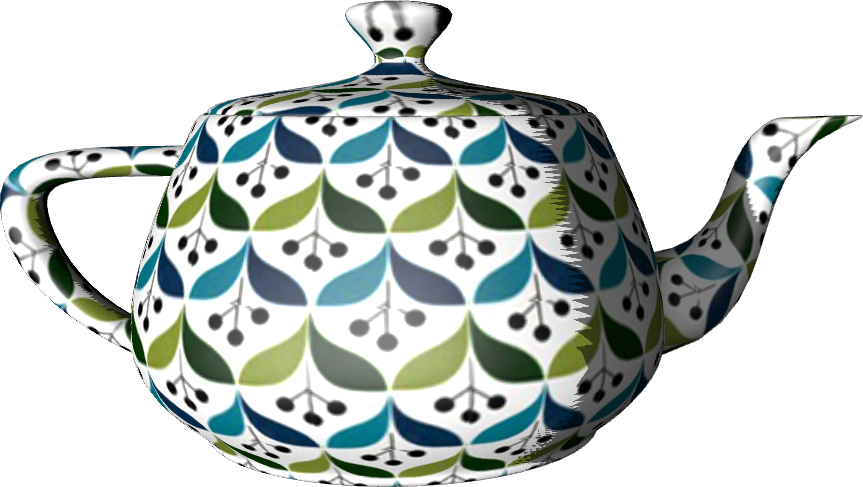
\includegraphics[width=0.48\textwidth]{kap5/figures/realism-x3dom.png}
		\label{FIG:REALISM_TEST_X3DOM}
	}
	\hfill
	\subfloat[WebGL]{
		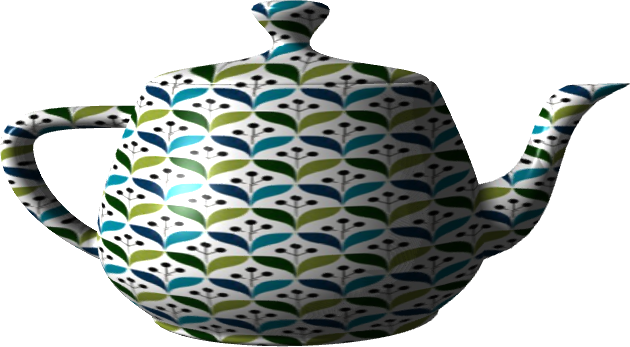
\includegraphics[width=0.48\textwidth]{kap5/figures/realism-webgl.png}
		\label{FIG:REALISM_TEST_WEBGL}
	}
	\caption{Vergleich der texturierten 3D-Modelle.}
	\label{FIG:REALISM_TEST}
\end{figure}

Abbildung \ref{FIG:REALISM_TEST} zeigt das jeweilige Resultat des mit einem Muster texturierten 3D-Modells. Beide Frameworks unterstützen Smooth-Shading mit einer diffusen und spekularen Reflexion. Hierdurch wird eine glatte Oberfläche der Teekane mit Glanzeffekten erzielt. Auch Schatten kann in beiden Ansätzen realisiert werden. Dabei zeigt sich jedoch ein Unterschied hinsichtlich der Qualität der Darstellung. Bei genauer Betrachtung der Schattenkontur in Abbildung \ref{FIG:REALISM_TEST_X3DOM} zeigt sich, anders als bei WebGL, kein weicher Übergang der Schattierung, sondern eine harte, ausgefranste Kante. Generell wirkt das mit Three.js gerenderte 3D-Modell hierdurch visuell ansprechender.

\subsection{Entwicklungs-Aufwand}

Aus den in Anforderung \ref{SEC:DEVELOPMENT_EFFORT} ausgeführten Gründen ist auch der Entwicklungsaufwand ein wichtiger zu bedenkender Faktor für die Umsetzung einer Web3D-Anwendung. Die bisherigen Beispiele und Erläuterungen veranschaulichen gut die paradigmatisch grundverschiedene Vorgehensweise des deklarativen (X3DOM) und des imperativen (WebGL) Vertreters von Web3D.

Während X3D durch den XML-basierten Aufbau eine sehr hohe Konvergenz zu gut verstandenen Webtechnologien wie HTML aufweist, stellt WebGL einen typischen Webentwickler aufgrund des sehr niedrigen Abstraktionsniveaus der Bibliothek vor anspruchsvollere Konzepte \autocite{Jankowski:2013:DII:2466533.2466547}. Die große Nähe zu Open GL ES erfordert ein weitaus tiefgreiferendes Verständis für die theoretischen Grundlagen der Computergrafik, als es X3D durch seinen deklarativen Stil verlangt. Populäre WebGL-Frameworks wie das behandelte Three.js können diese Hürde zwar durch Abstraktion der Funktionalität deutlich senken, dennoch ist der Einarbeitungsaufwand bei WebGL höher einzustufen.

\section{Bewertung der Testergebnisse}

Die Browser- und Plattformunterstützung ist bei beiden Technologien durch das WebGL-Backend von X3DOM sehr ähnlich. Wie Tabelle \ref{TAB_BROWSER_SUPPORT} zeigt, steht WebGL und damit auch X3D in nazu allen aktuellen Browser-Versionen zur Verfügung. Wie ausgeführt besitzt X3DOM ein ausgereiftes Fallback-System und kann bei Bedarf dynamisch auf das weit verbreitete Flash-Plugin umschalten. Hierdurch können auch Benutzer des Internet Explorers 9 und 10 adressiert werden, woraus eine größere generelle Browserunterstützung resultiert. Mit der Veröffentlichung von iOS 8 im Herbst 2014 wird zudem auch eine der letzten verbleibenden Plattformen eine Unterstützung für WebGL erhalten.

Wie der Vergleich der Hardware-Anforderungen zeigt, ist WebGL zumindest innerhalb des betrachteten Testfalls, also bei vielen Geometrien in einer Szene, leistungstechnisch X3DOM überlegen. Bezogen auf die exemplarischen Anwendungsfälle, welche zu Beginn der Anforderungsanalyse in Abschnitt \ref{SEC:APPLICATION_DOMAIN} beschrieben wurden, würde dieser Fall bespielsweise bei der Darstellung komplexer wissenschaftlicher Abbildungen mit sehr vielen Einzelelementen auftreten. Bei Betrachtung eines einzelnen Produkts tritt dieser Aspekt hingegen in den Hintergrund und andere Kriterien wie der Entwicklungsaufwand und die generelle Einfachheit bei der Umsetzung gewinnen an Bedeutung. Hinsichtlich dieser Kriterien ist X3DOM gegenüber WebGL aufgrund seines deklarativen Ansatzes zu bevorzugen. Im Gegensatz zu WebGL, welches ein zumindest grundlegendes Verständnis computergrafischer Konzepte und der Grafik-Pipeline erfordert, sind hier bereits wenige HTML-Kenntnisse ausreichend, um eine 3D-Szene mittels X3DOM umzusetzen.

Beide Frameworks ermöglichen das Importieren einiger offener 3D-Grafikformate, sodass bestehende 3D-Modelle problemlos eingebunden werden können. Dabei ist gegebenfalls eine Umwandlung des Ausgangsmodells in ein durch X3DOM beziehungsweise Three.js unterstütztes Format durch Modellierungssoftware wie Blender \autocite{SOFTWARE_BLENDER} notwendig. Durch die Unterstützung der gängigen Beleuchtungs-Modelle, Shading-Verfahren und Texturierung verhalten sich beide Ansätze hinsichtlich der realistischen Darstellung von 3D-Modellen ähnlich. X3DOM wies innerhalb des Tests hier jedoch einige Artefakte bei der Schattenkontur auf. Die spezifizierten Anforderungen bezüglich der Benutzerinterkation können in beiden Technologien gleich gut realisiert werden.

	\chapter{Zusammenfassung}

Seit dem Aufkommen der Web Graphics Library im Jahr 2009 ist eine neue Dynamik im Web3D-Umfeld entstanden. Mit der heutigen Verfügbarkeit von WebGL in nahezu jedem Webbrowser ist die Darstellung hardwarebeschleunigter 3D-Grafik heute ohne Plugins möglich. Mit X3DOM hat sich innerhalb der letzten Jahre ein umfangreiches JavaScript-Framework entwickelt, welches die Nutzung des freien X3D-Standards zur Deklaration von 3D-Szenen in HTML ermöglicht. Behr et al. erhoffen sich, langfristig eine native Unterstützung von X3D innerhalb der Browser ähnlich zu SVG zu erzielen. Auch auf Seite von WebGL sind seit dessen Erscheinung eine Vielzahl von Frameworks entstanden, welche die Programmierung anspruchsvoller 3D-Anwendungen mit großer Flexibilität erlauben. Durch Abstraktion der Funktionaliät der Hardware-nahen Grafikbibliothek wird deren Benutzung stark vereinfacht.

Wie die Evaluation gezeigt hat, ähneln sich X3DOM und WebGL in vielen Aspekten wie der Browser- und Plattformunterstützung und den Möglichkeiten hinsichtlich der Benutzerinteraktion sehr. Auch der Import bestehender 3D-Daten ist bei beiden Ansätzen einfach zu realisieren. Der hauptsächliche Unterschied der zwei betrachteten Technologien liegt in ihrer paradigmatischen Grundlage. Zwar ermöglicht es der deklarative Stil von X3DOM sehr leicht, 3D-Szenen auch ohne Programmierkenntnisse umzusetzen, jedoch schränkt dies die Flexiblität des Entwicklers gleichzeitig ein, da nicht jeder Aspekt der Darstellung bis ins letzte Detail beeinflusst werden kann. Je nach konkreter Anwendung und Vorwissen des Software-Entwicklers muss die Wahl der 3D-Technologie somit von Fall zu Fall entschieden werden.

Die von Ortiz 2010 hauptsächlich gesehenen Probleme, die Web3D davon abhalten, sich im WWW stärker zu etablieren, -- der Mangel an Standardisierung und die Notwendigkeit von Browser-Plugins -- können im Jahr 2014 als überwunden betrachtet werden. Es bleibt abzuwarten, inwieweit sich WebGL in den nächsten Jahren weiterentwickeln wird und ob es X3D ebenso schaffen wird, eine native Unterstützung innerhalb der Webbrowser zu erreichen.

	\newpage
	\pagenumbering{Roman}


	\begingroup
	\raggedright
	\sloppy
	\addchap{Quellenverzeichnis}
	\printbibliography[title={Literatur}, nottype=online, notkeyword=software, heading=subbibliography]
	\printbibliography[title={Online-Quellen},type=online,notkeyword=software, heading=subbibliography]
	\printbibliography[title={Software},keyword=software, heading=subbibliography]
	\endgroup


	\listoffigures
	\begingroup
	\let\clearpage\relax
	\listoftables
	\endgroup

	\addchap{Eidesstattliche Erklärung}

Hiermit versichere ich, dass ich die vorliegende Bachelorarbeit selbständig verfasst habe. Ich versichere, dass ich keine anderen als die angegebenen Quellen benutzt und alle wörtlich oder sinngemäß aus anderen Werken übernommenen Aussagen als solche gekennzeichnet habe, und dass die eingereichte Arbeit weder vollständig noch in wesentlichen Teilen Gegenstand eines anderen Prüfungsverfahren gewesen ist.

Erlangen, den \today
\vspace{0.5cm}

\makebox[4cm]{\hrulefill}
\newline\vspace{1cm}
Jonathan Gruber

	\begin{appendix}
		\chapter{Quelltext der Beispiel-Anwendung}

\section{X3DOM}
\label{APPENDIX:X3DOM_EXAMPLE}
\htmlinput[fontsize=\scriptsize]{kap4/x3d/example/index.html}

\section{WebGL}
\label{APPENDIX:WEBGL_EXAMPLE}
\jsinput[fontsize=\scriptsize]{kap4/webgl/example/main.js}

\chapter{Quelltext der Testumgebung}

Aufgrund des Umfangs der implementierten Testumgebung wird deren Quelltext hier nicht abgedruckt, sondern liegt lediglich digital auf der beigefügten CD vor.
Der vollständige Quellcode wurde jedoch zusätzlich in ein GitHub-Repository hochgeladen. Dieses ist unter folgender Adresse zu erreichen:

\url{https://github.com/gruberjonathan/web3d}

Die Testumgebung ist zusätzlich unter folgender Adresse online verfügbar:

\url{http://web3d.webreaktor.net}

	\end{appendix}
\end{document}
